% Judul dokumen
\title{Buku Tugas Akhir ITS}
\author{Fahreza, Dimas Iqbal}

% Pengaturan ukuran teks dan bentuk halaman dua sisi
\documentclass[12pt,twoside]{report}

% Pengaturan ukuran halaman dan margin
\usepackage[a4paper,top=30mm,left=30mm,right=20mm,bottom=25mm]{geometry}

% Pengaturan ukuran spasi
\usepackage[singlespacing]{setspace}

% Pengaturan format bahasa
\usepackage[indonesian]{babel}

% Pengaturan detail pada file PDF
\usepackage[pdfauthor={\@author},bookmarksnumbered,pdfborder={0 0 0}]{hyperref}

% Pengaturan jenis karakter
\usepackage[utf8]{inputenc}

% Pengaturan pewarnaan
\usepackage[table,xcdraw]{xcolor}

% Pengaturan kutipan artikel
\usepackage[square,numbers]{natbib}

% Package lainnya
\usepackage{changepage}
\usepackage{enumitem}
\usepackage{eso-pic}
\usepackage{etoolbox}
\usepackage{graphicx}
\usepackage{lipsum}
\usepackage{lmodern}
\usepackage{longtable}
\usepackage{tabularx}
\usepackage{wrapfig}
\usepackage{tikz}
\usepackage{adjustbox}
\usepackage{multirow}

% Definisi untuk "Hati ini sengaja dikosongkan"
\patchcmd{\cleardoublepage}{\hbox{}}{
  \thispagestyle{empty}
  \vspace*{\fill}
  \begin{center}\textit{[Halaman ini sengaja dikosongkan]}\end{center}
  \vfill}{}{}

% Pengaturan penomoran halaman
\usepackage{fancyhdr}
\fancyhf{}
\renewcommand{\headrulewidth}{0pt}
\pagestyle{fancy}
\fancyfoot[RE,RO]{\thepage}
\patchcmd{\chapter}{plain}{fancy}{}{}
\patchcmd{\chapter}{empty}{plain}{}{}

% Pengaturan format judul bab
\usepackage{titlesec}
\titleformat{\chapter}[display]{\bfseries\Large}{BAB \centering\Roman{chapter}}{0ex}{\vspace{0ex}\centering}
\titleformat{\section}{\bfseries\large}{\MakeUppercase{\thesection}}{1ex}{\vspace{1ex}}
\titleformat{\subsection}{\bfseries\large}{\MakeUppercase{\thesubsection}}{1ex}{}
\titleformat{\subsubsection}{\bfseries\large}{\MakeUppercase{\thesubsubsection}}{1ex}{}
\titlespacing{\chapter}{0ex}{0ex}{4ex}
\titlespacing{\section}{0ex}{1ex}{0ex}
\titlespacing{\subsection}{0ex}{0.5ex}{0ex}
\titlespacing{\subsubsection}{0ex}{0.5ex}{0ex}

% Pengaturan format potongan kode
\usepackage{listings}
\definecolor{comment}{RGB}{0,128,0}
\definecolor{string}{RGB}{255,0,0}
\definecolor{keyword}{RGB}{0,0,255}
\lstdefinestyle{codestyle}{
  commentstyle=\color{comment},
  stringstyle=\color{string},
  keywordstyle=\color{keyword},
  basicstyle=\footnotesize\ttfamily,
  numbers=left,
  numberstyle=\tiny,
  numbersep=5pt,
  frame=lines,
  breaklines=true,
  prebreak=\raisebox{0ex}[0ex][0ex]{\ensuremath{\hookleftarrow}},
  showstringspaces=false,
  upquote=true,
  tabsize=2,
}
\lstset{style=codestyle}

% Isi keseluruhan dokumen
\begin{document}

  % Sampul luar Bahasa Indonesia
  \newcommand\covercontents{sampul/konten-id.tex}
  \input{sampul/sampul-luar.tex}

  % Atur ulang penomoran halaman
  \setcounter{page}{1}

  % Sampul dalam Bahasa Indonesia
  \renewcommand\covercontents{sampul/konten-id.tex}
  \input{sampul/sampul-dalam.tex}
  \clearpage
  \cleardoublepage

  % Sampul dalam Bahasa Inggris
  \renewcommand\covercontents{sampul/konten-en.tex}
  \input{sampul/sampul-dalam.tex}
  \cleardoublepage

  % Pengaturan ukuran indentasi paragraf
  \setlength{\parindent}{2em}

  % Pengaturan ukuran spasi paragraf
  \setlength{\parskip}{1ex}

  % Lembar pengesahan
  \begin{center}
	\large
  \textbf{LEMBAR PENGESAHAN}
\end{center}

% Menyembunyikan nomor halaman
\thispagestyle{empty}

\begin{center}
  % Ubah kalimat berikut dengan judul tugas akhir
  \textbf{KLASIFIKASI GENRE DAN SUBGENRE MUSIK BERBASIS FITUR MEL-FREQUENCY CEPSTRAL COEFFICIENTS MENGGUNAKAN CONVOLUTIONAL NEURAL NETWORK}
\end{center}

\begingroup
  % Pemilihan font ukuran small
  \small
  
  \vspace{3ex}

  \begin{center}
    \textbf{PROPOSAL TUGAS AKHIR}
    \\Diajukan untuk memenuhi salah satu syarat
    \\memperoleh gelar Sarjana Teknik pada
    \\Program Studi S-1 Teknik Komputer
    \\Departemen Teknik Komputer
    \\Fakultas Teknologi Elektro dan Informatika Cerdas
    \\Institut Teknologi Sepuluh Nopember
  \end{center}

  \vspace{3ex}

  \begin{center}
    % Ubah kalimat berikut dengan nama dan NRP mahasiswa
    Oleh: Dimas Iqbal Fahreza
    \\NRP. 0721 18 4000 0045
  \end{center}

  \vspace{3ex}

  % \begin{center}
  % Ubah kalimat-kalimat berikut dengan tanggal ujian dan periode wisuda
  %   Tanggal Ujian : 1 Juni 2021\\
  %   Periode Wisuda : September 2021
  % \end{center}

  \begin{center}
    Disetujui oleh Tim Penguji Tugas Akhir:
  \end{center}

  \vspace{4ex}

  \begingroup
    % Menghilangkan padding
    \setlength{\tabcolsep}{0pt}

    \noindent
    \begin{tabularx}{\textwidth}{X l}
      % Ubah kalimat-kalimat berikut dengan nama dosen pembimbing pertama
      1. Reza Fuad Rachmadi, S.T., M.T., Ph.D.          & Pembimbing \\
      % NIP: 18560710 194301 1 001        & ................................... \\
      &  \\
      &  \\
      % Ubah kalimat-kalimat berikut dengan nama dosen pembimbing kedua
      2. Dr. Eko Mulyanto Yuniarno, S.T., M.T.     & Ko-Pembimbing \\
      &  \\
      &  \\
      % Ubah kalimat-kalimat berikut dengan nama dosen penguji pertama
      3. Dr. Galileo Galilei, S.T., M.Sc.  & Penguji I \\
      &  \\
      &  \\
      % Ubah kalimat-kalimat berikut dengan nama dosen penguji kedua
      4. Friedrich Nietzsche, S.T., M.Sc.  & Penguji II \\
      &  \\
      &  \\
      % Ubah kalimat-kalimat berikut dengan nama dosen penguji ketiga
      5. Alan Turing, ST., MT.             & Penguji III \\
      &  \\
      &  \\
    \end{tabularx}
  \endgroup

  \vspace{12ex}

  % \begin{center}
  %   % Ubah kalimat berikut dengan jabatan kepala departemen
  %   Mengetahui, \\
  %   Kepala Departemen Teknik Dirgantara FTD - ITS \\

  %   \vspace{8ex}

  %   % Ubah kalimat-kalimat berikut dengan nama dan NIP kepala departemen
  %   \underline{Dr. Leonardo Da Vinci, S.T., M.T.} \\
  %   NIP. 14520415 151905 1 001
  % \end{center}

  \begin{center}
    \textbf{SURABAYA\\Mei, 2022}
  \end{center}
\endgroup

  \cleardoublepage

  % Pernyataan keaslian
  \begin{center}
  \large
  \textbf{PERNYATAAN ORISINALITAS}
\end{center}

% Menyembunyikan nomor halaman
\thispagestyle{empty}

\vspace{2ex}

% Ubah paragraf-paragraf berikut sesuai dengan yang ingin diisi pada pernyataan keaslian

\noindent Yang bertanda tangan dibawah ini:

\noindent\begin{tabularx}{\textwidth}{X X l}
  & \\
  Nama Mahasiswa / NRP &: Dimas Iqbal Fahreza / 0721 18 4000 0045 \\
  Departemen &: Teknik Komputer \\
  Dosen Pembimbing &: Reza Fuad Rachmadi, S.T., M.T., Ph.D \\
  & \\
\end{tabularx}

Dengan ini menyatakan bahwa Tugas Akhir dengan judul "Klasifikasi Genre Dan Subgenre Musik Berbasis Fitur MFCC Menggunakan CNN" adalah hasil karya sendiri, berfsifat orisinal, dan ditulis dengan mengikuti kaidah penulisan ilmiah.

Bilamana di kemudian hari ditemukan ketidaksesuaian dengan pernyataan ini, maka saya bersedia menerima sanksi sesuai dengan ketentuan yang berlaku di Institut Teknologi Sepuluh Nopember.

\vspace{8ex}

\noindent\begin{tabularx}{\textwidth}{X l}
  % Ubah kalimat berikut sesuai dengan tempat, bulan, dan tahun penulisan
  & Surabaya, Mei 2022\\
  & \\
  Mengetahui & \\
  Dosen Pembimbing & Mahasiswa\\
  & \\
  & \\
  & \\
  & \\
  & \\
  (Reza Fuad Rachmadi, S.T., M.T., Ph.D) & (Dimas Iqbal Fahreza) \\
  NIP. 19850403201212 1 000& NRP. 0721 18 4000 0045\\
\end{tabularx}
  \cleardoublepage

  % Nomor halaman pembuka dimulai dari sini
  \pagenumbering{roman}

  % Abstrak Bahasa Indonesia
  \begin{center}
  \large\textbf{ABSTRAK}
\end{center}

\addcontentsline{toc}{chapter}{ABSTRAK}

\vspace{2ex}

\begingroup
  % Menghilangkan padding
  \setlength{\tabcolsep}{0pt}

  \noindent
  \begin{tabularx}{\textwidth}{l >{\centering}m{2em} X}
    % Ubah kalimat berikut dengan nama mahasiswa
    Nama Mahasiswa    &:& Dimas Iqbal Fahreza \\

    % Ubah kalimat berikut dengan judul tugas akhir
    Judul Tugas Akhir &:&	Klasifikasi Genre Dan Subgenre Musik Berbasis Fitur Mel-frequency Cepstral Coefficients Menggunakan Convolutional Neural Network \\

    % Ubah kalimat-kalimat berikut dengan nama-nama dosen pembimbing
    Pembimbing        &:& 1. Reza Fuad Rachmadi, S.T., M.T., Ph.D \\
                      & & 2. Dr. Eko Mulyanto Yuniarno, S.T., M.T. \\
  \end{tabularx}
\endgroup

% Ubah paragraf berikut dengan abstrak dari tugas akhir
Dewasa ini, dengan semakin banyaknya musik yang diunggah ke internet, serta 
perkembangan platform untuk mendengarkan musik secara daring, seperti Spotify, 
Bandcamp, Deezer, SoundCloud, dan lain sebagainya, pengguna dapat mendengarkan musik 
yang mereka sukai dimana saja dan kapan saja. Jumlah musik yang sangat banyak tersebut 
perlu untuk dikategorikan berdasarkan genrenya secara otomatis karena sangatlah tidak 
mungkin bagi manusia untuk melakukannya secara manual. Oleh karena itu, diperlukan 
suatu sistem klasifikasi genre dan subgenre musik berbasis deep learning agar pengkategorian genre dan subgenre musik dapat dilakukan dengan lebih cepat dan akurat. Musik yang diklasifikasikan akan dilakukan 
teknik algoritma Mel-Frequency Coefficient of Cepstrum (MFCC), serta menggunakan model 
Convolutional Neural Network (CNN). 

% Ubah kata-kata berikut dengan kata kunci dari tugas akhir
Kata Kunci: Klasifikasi, Subgenre, MFCC, CNN

  \cleardoublepage

  % Abstrak Bahasa Inggris
  \begin{center}
  \large\textbf{ABSTRACT}
\end{center}

\addcontentsline{toc}{chapter}{ABSTRACT}

\vspace{2ex}

\begingroup
  % Menghilangkan padding
  \setlength{\tabcolsep}{0pt}

  \noindent
  \begin{tabularx}{\textwidth}{l >{\centering}m{3em} X}
    % Ubah kalimat berikut dengan nama mahasiswa
    \emph{Name}     &:& Dimas Iqbal Fahreza \\

    % Ubah kalimat berikut dengan judul tugas akhir dalam Bahasa Inggris
    \emph{Title}    &:& \emph{Music Genre And Subgenre Classification Based on Mel-frequency Cepstral Coefficients Features Using Convolutional Neural Network} \\

    % Ubah kalimat-kalimat berikut dengan nama-nama dosen pembimbing
    \emph{Advisors} &:& 1. Reza Fuad Rachmadi, S.T., M.T., Ph.D \\
                    & & 2. Dr. Eko Mulyanto Yuniarno, S.T., M.T. \\
  \end{tabularx}
\endgroup

% Ubah paragraf berikut dengan abstrak dari tugas akhir dalam Bahasa Inggris
\emph{In this research, we proposed \lipsum[1]}

% Ubah kata-kata berikut dengan kata kunci dari tugas akhir dalam Bahasa Inggris
\emph{Keywords}: \emph{Rocket}, \emph{Anti-gravity}, \emph{Energy}, \emph{Space}.

  \cleardoublepage

  % Kata pengantar
  \begin{center}
  \Large
  \textbf{KATA PENGANTAR}
\end{center}

\addcontentsline{toc}{chapter}{KATA PENGANTAR}

\vspace{2ex}

% Ubah paragraf-paragraf berikut dengan isi dari kata pengantar

Puji dan syukur kehadirat Tuhan Yang Maha Esa atas segala karunia-Nya, penulis dapat menyelesaikan penelitian ini yang berjudul \textbf{Klasifikasi Genre Dan Subgenre Musik Berbasis Fitur Mel-frequency Cepstral Coefficients Menggunakan Convolutional Neural Network (\emph{Music Genre And Subgenre Classification Based on Mel-frequency Cepstral Coefficients Features Using Convolutional Neural Network})}.

 Penelitian ini disusun dalam rangka memenuhi bidang riset di Departemen Teknik Komputer ITS serta digunakan sebagai persyaratan menyelesaikan pendidikan S1. Oleh karena itu, penulis mengucapkan terima kasih kepada:

\begin{enumerate}[nolistsep]

  \item Keluarga, Ibu, Bapak dan Saudara tercinta yang telah memberikan segala bentuk dukungan

  \item Bapak Reza Fuad Rachmadi, S.T., M.T., selaku dosen pembimbing 1

   \item Bapak Dr. Eko Mulyanto Yuniarno, S.T., M.T., selaku dosen pembimbing 2
   
   \item Bapak-ibu dosen pengajar Departemen Teknik Komputer ITS atas segala ilmu dan arahannya
   
   \item Teman-teman Asisten Lab B201 yang telah menemani dan mendukung
   
   \item Serta teman-teman Teknik Komputer angkatan 2018 yang telah bersama-sama menempuh segala kegiatan perkuliahan dari awal sampai akhir masa kuliah penulis

\end{enumerate}

Kesempurnaan hanya milik Tuhan Yang Maha Esa, untuk itu
penulis memohon segenap kritik dan saran yang membangun. Semoga penelitian ini dapat memberikan manfaat bagi kita semua.
Amin.

\begin{flushright}
  \begin{tabular}[b]{c}
    % Ubah kalimat berikut dengan tempat, bulan, dan tahun penulisan
    Surabaya, Mei 2022\\
    \\
    \\
    \\
    \\
    % Ubah kalimat berikut dengan nama mahasiswa
    Penulis
  \end{tabular}
\end{flushright}

  \cleardoublepage

  % Daftar isi
  \renewcommand*\contentsname{DAFTAR ISI}
  \addcontentsline{toc}{chapter}{\contentsname}
  \tableofcontents
  \cleardoublepage

  % Daftar gambar
  \renewcommand*\listfigurename{DAFTAR GAMBAR}
  \addcontentsline{toc}{chapter}{\listfigurename}
  \listoffigures
  \cleardoublepage

  % Daftar tabel
  \renewcommand*\listtablename{DAFTAR TABEL}
  \addcontentsline{toc}{chapter}{\listtablename}
  \listoftables
  \cleardoublepage

  % Nomor halaman isi dimulai dari sini
  \pagenumbering{arabic}

  % Bab 1 pendahuluan
  \chapter{PENDAHULUAN}
\label{chap:pendahuluan}

% Ubah bagian-bagian berikut dengan isi dari pendahuluan

\section{Latar Belakang}
\label{sec:latarbelakang}

Genre musik adalah metode pengkategorian untuk mengidentifikasikan suatu musik ke dalam suatu tradisi yang sudah pernah ada \citep{Genre}. Musik dapat dibedakan menjadi berbagai macam genre, seperti Pop, Rock, Blues, Jazz, Religi, dan lain sebagainya. Sifat dari musik sendiri adalah subjektif sehingga klasifikasi genre tiap orang bisa jadi berbeda-beda dan mungkin juga ada beberapa genre yang saling tumpang tindih satu sama lain.

Penyebaran penggunaan internet telah membawakan perubahan yang besar pada dunia industri permusikan. Perubahan-perubahannya adalah seperti menyebarnya platform untuk mendengarkan musik secara daring, serta klasifikasi genre musik yang kemudian digunakan sebagai sistem rekomendasi. Dewasa ini, dengan perkembangan platform untuk mendengarkan musik secara daring, pengguna dapat mendengarkan musik yang mereka sukai dimana saja dan kapan saja, serta mereka dapat mencari jutaan musik melalui platform-platform tersebut, seperti Spotify, Bandcamp, Deezer, SoundCloud, dan lain sebagainya \citep{Elbir2018MusicGC}.

Pada hari Senin, 22 Februari 2021, Spotify telah mengkonfirmasi bahwa lebih dari 60.000 trek baru diunggah ke platformnya setiap hari. Menurut Jeremy Elrich, co-Head of Music dari Spotify, hal ini berarti pada akhir tahun ini dapat diperkirakan terdapat 22 juta trek musik yang akan ditambahkan ke katalog musik Spotify. Dengan angka 60.000 per hari, dapat dihitung bahwa setiap 1,4 detik terdapat satu trek baru yang diunggah. Spotify mengkonfirmasi bahwa pada bulan November tahun lalu, platform tersebut memiliki sekitar 70 juta trek yang tersimpan di dalamnya, dari sini maka dapat diperkirakan bahwa pada akhir tahun ini Spotify akan menjadi rumah untuk lebih dari 90 juta trek musik, dan akan menjadi lebih dari 100 juta pada awal tahun berikutnya \citep{musicb}.

\section{Permasalahan}
\label{sec:permasalahan}

Dengan semakin banyaknya musik yang diunggah tiap harinya, maka sangatlah tidak mungkin bagi manusia untuk mengkategorikan musik yang telah diunggah ke genre yang sesuai secara manual. Oleh karena itu, diperlukan deep learning untuk klasifikasi genre musik agar proses pengkategorian musik dapat dilakukan dengan lebih cepat dan akurat.

\section{Batasan Masalah}
\label{sec:batasanmasalah}

Batasan-batasan dari \lipsum[1][1-3] adalah:

\begin{enumerate}[nolistsep]

  \item Mempermudah \lipsum[2][1-3]

  \item \lipsum[3][1-5]

  \item \lipsum[4][1-5]

\end{enumerate}

\section{Tujuan}
\label{sec:Tujuan}

Penelitian ini bertujuan untuk membuat suatu sistem yang dapat mengklasifikasikan beberapa subgenre yang paling masuk akal dari suatu input data musik yang diambil dari genre yang berbeda-beda serta dengan durasi yang relatif fleksibel. Sistem klasifikasi ini dilakukan dengan menggunakan Mel-frequency cepstral coefficients (MFCC) sebagai fitur utama serta Convolutional Neural Network (CNN) sebagai framework deep learning-nya.

\section{Manfaat}
\label{sec:manfaat}

Manfaat dari \lipsum[1][1-3] adalah:

\begin{enumerate}[nolistsep]

  \item Mempermudah \lipsum[2][1-3]

  \item \lipsum[3][1-5]

  \item \lipsum[4][1-5]

\end{enumerate}

% Format Buku TA baru, ga pake sistematika penulisan

% \section{Sistematika Penulisan}
% \label{sec:sistematikapenulisan}

% Laporan penelitian tugas akhir ini terbagi menjadi \lipsum[1][1-3] yaitu:

% \begin{enumerate}[nolistsep]

%   \item \textbf{BAB I Pendahuluan}

%   Bab ini berisi \lipsum[2][1-5]

%   \vspace{2ex}

%   \item \textbf{BAB II Tinjauan Pustaka}

%   Bab ini berisi \lipsum[3][1-5]

%   \vspace{2ex}

%   \item \textbf{BAB III Desain dan Implementasi Sistem}

%   Bab ini berisi \lipsum[4][1-5]

%   \vspace{2ex}

%   \item \textbf{BAB IV Pengujian dan Analisa}

%   Bab ini berisi \lipsum[5][1-5]

%   \vspace{2ex}

%   \item \textbf{BAB V Penutup}

%   Bab ini berisi \lipsum[6][1-5]

% \end{enumerate}

  \cleardoublepage

  % Bab 2 tinjauan pustaka
  \chapter{TINJAUAN PUSTAKA}
\label{chap:tinjauanpustaka}

% Ubah bagian-bagian berikut dengan isi dari tinjauan pustaka

\section{Penelitian Terdahulu}
\label{sec:penelitianterdahulu}

Untuk mengklasifikasikan suatu musik dapat dilakukan dengan cara membedakan dari genre dan atau subgenrenya. Berikut adalah penelitian terdahulunya.

\subsection{Klasifikasi Genre}

Pandu Deski Prasetyo dkk. \citep{prasetyo} menggunakan dataset buatan sendiri yang berisikan 250 berkas musik yang terbagi menjadi genre pop, rock, dangdut, jazz, dan folk. Masing-masing genre memiliki sampel data sebanyak 50 berkas musik. Metode yang digunakan adalah Mel-Frequency Cepstrum Coefficients dengan k-Nearest Neighbors sebagai classifier-nya. Hasil akurasi yang diperoleh dengan k = 13 adalah sebanyak 52.4%.

Hareesh Bahuleyan \citep{DBLP:journals/corr/abs-1804-01149} menggunakan dataset Audio Set yang dimana merupakan hasil dari ekstraksi klip suara 10 detik dari total 2,1 juta video YouTube. Klip suara tersebut berisikan bermacam-macam suara seperti instrumen musik, suara kendaraan, suara hewan, dan lain sebagainya. Namun, yang digunakan pada penelitian itu hanyalah suara berkategori musik dengan total 40.540 klip suara musik dengan genre-genre seperti Pop, Rock, Hip Hop, Techno, Rhythm Blues, Vocal, dan Reggae. Metode yang digunakan adalah dengan membuat Mel-Spektrogram dari klip suara yang kemudian menggunakan model Convolutional Neural Network (CNN), serta berbagai macam classifier, seperti Logistic Regression (LR), Random Forest (RF), Gradient Boosting (XGB), serta Support Vector Machines (SVM). Hasil akurasi yang diperoleh dengan metode CNN Transfer Learning sebanyak 63\%, CNN Fine Tuning sebanyak 64\%, LR sebanyak 53\%, RF sebanyak 54\%, SVM sebanyak 57\% XGB sebanyak 59\%, dan gabungan CNN dengan XGB sebanyak 65\%.

Michael Haggblade dkk. \citep{Haggblade2011MusicGC} menggunakan dataset GTZAN Genre Collection yang berisikan 1000 trek musik dengan durasi masing-masing sepanjang 30 detik. Terdapat 10 genre pada dataset tersebut dengan masing-masing 100 trek. Pada penelitian itu, hanya digunakan 4 genre (Classical, Jazz, Metal, dan Pop) dengan total 400 trek musik. Metode yang digunakan adalah Mel-Frequency Cepstrum Coefficients dengan k-Nearest Neighbors, k-Means, DAG SVM, dan Neural Network sebagai classifier-nya. Hasil akurasi yang diperoleh dengan urutan genre Classical, Jazz, Metal, dan Pop dengan metode DAG SVM sebanyak 97\%, 67\%, 87\%, dan 97\%, Neural Network sebanyak 88\%, 100\%, 76\%, dan 100\%, k-Means sebanyak 88\%, 61\%, 93\%, dan 90\%, serta k-NN sebanyak 87\%, 67\%, 80\%, dan 90\%.

\subsection{Klasifikasi Subgenre}
Quinto dkk \citep{quinto} menggunakan dataset yang berisikan 3 subgenre dari musik bergenre jazz, yaitu Swing/Electroswing, Bebop, dan Acid Jazz. Total durasi per subgenrenya adalah 254 menit untuk Acid Jazz, 141 menit untuk Bebop, dan 245 menit untuk Swing sehingga terdapat imbalance terhadap Bebop. Sample rate yang digunakan adalah 22050Hz mono. Setiap potongan musik dilakukan segmentasi menjadi 10 detik, dengan fitur yang diekstraksi adalah MFCC. Metode yang digunakan adalah SVM, KNN, MLP, dan LSTM dengan masing-masing akurasi tertingginya adalah secara berurutan 81,67\%, 77,43\%, 79,39\%, dan 89,824\%.

Tsatsishvili \cite{tsatsishvili} menggunakan dataset yang berisikan 7 subgenre dari musik bergenre heavy metal dengan total 210 trek. Masing-masing subgenre memiliki 30 trek. Subgenre yang digunakan adalah black, death, melodic death, gothic, heavy, power, dan progressive metal. Fitur-fitur audio yang diekstraksi adalah seperti timbral, rhythmic, dynamic, dan pitch information. Metode yang mendapatkan akurasi tertinggi adalah dengan AdaBoost dan J48 classifier menggunakan fitur spectral yang hasilnya 45,7\%.

Mulder \citep{Mulder2014AutomaticCO}  menggunakan dataset yang berisikan 17 subgenre dari musik bergenre heavy metal dengan total 646 trek. Masing-masing subgenre memiliki 38 trek. Subgenre yang digunakan adalah seperti alternative metal, black metal, classic metal, death metal, doom metal, folk metal, gothic metal, groove metal, industrial metal, melodeath metal, nu metal, power metal, progressive metal, sludge metal, stoner metal, symphonic metal, dan thrash metal. Fitur audio yang digunakan sebagai klasifikasi adalah chroma, horizontal dan vertical musical interval. Metode yang digunakan adalah k-NN classifier. Akurasi yang didapat menggunakan classifier terbaiknya adalah 28\% untuk fitur vertical interval dan 21\% untuk fitur horizontal interval.

\section{Musik}
\label{sec:musik}
Setiap musik pasti berbeda, namun meskipun berbeda mereka masih disebut sebagai musik. Musik bukanlah sekedar sesuatu yang enak untuk didengar, dibaliknya terdapat tradisi yang sangat mendalam layaknya seperti sebuah bahasa. Tidak ada budaya yang tidak memiliki bahasa, begitu pula tidak ada budaya yang tidak memiliki musik. Biasanya, orang hanya memerlukan beberapa detik untuk menyadari genre yang direferensikan dari sebuah musik komersil, serta apa asosiasi dan konotasi dibaliknya. Tentunya, hal ini memerlukan pengalaman serta keakraban terhadap kultur tersebut. Karakter dari musik sangatlah berbeda tergantung pada daerah dan budayanya, musik berfungsi sebagai simbol dari identitas nasional maupun regional. Musik merupakan kata yang sangat kecil untuk menggambarkan sesuatu yang memiliki banyak bentuk serta identitas budaya maupun sub budaya \citep{cook1998music}.

\section{Genre}
\label{sec:genre}
Pada dasarnya, genre merupakan sebuah tipe pengkategorian suatu musik ke sebuah kultur tertentu. Sebuah genre tidaklah hanya berdasarkan pada musiknya itu sendiri, tapi juga pikiran serta kebiasaan dari grup tertentu yang memelihara suatu adat tersebut. Adat-adat ini dibuat bedasarkan pada teks musikal, artis, serta konteks tertentu yang kemudian dipertunjukkan serta dinikmati oleh kalangan adat itu sendiri. Dari sini dapat dikatakan bahwa genre merupakan struktur fundamental dari suatu musik yang mengimplikasikan bagaimana, dimana, dan siapa yang membuat dan menikmati musik tersebut. Genre akan terus berlanjut untuk meninggalkan jejak kultur dan sejarah sepanjang hidup. Sifat dari genre sendiri adalah kolektif, baik secara musikal, maupun sosial. Adat dan ekspektasi tertanam melalui repetisi yang dilakukan oleh kalangan tertentu, dan proses lahirnya suatu genre biasanya beriringan dengan lahirnya suatu kalangan sosial yang baru\citep{holt2007genre}.

\section{Subgenre}
\label{sec:subgenre}
Terdapat makna sosial, finansial, serta artistik yang dalam pada label untuk mengkategorikan subgenre dari musik, tidak hanya semata-mata untuk memisahkan musik yang terdengar berbeda. Seorang artis masih dapat mengkategorikan musik mereka ke dalam suatu subgenre yang baru, tapi hal ini tidak semudah itu untuk label rekaman. Untuk menambahkan subgenre baru diperlukan banyak pertimbangan, seperti untuk meningkatkan penjualan, sebagai agenda politik, atau untuk mengundang pendengar baru (maupun sebaliknya). Dikarenakan pengkategorian label subgenre bukanlah hal yang mudah dan memerlukan banyak pertimbangan yang kompleks, penataan hierarki dari subgenre musik lebih sulit dibandingkan dengan genre. Terbatasnya akses dataset untuk melakukan penelitian klasifikasi subgenre menjadi sebuah kesulitan utama. Hal ini terjadi karena kurangnya penelitian klasifikasi subgenre di ranah Music Information Retrieval (MIR) \citep{lefaivre2019characterizing}.

\section{Machine Learning}
\label{sec:machinelearning}

% Contoh penggunaan referensi dari pustaka
% Newton pernah merumuskan \citep{Newton1687} bahwa \lipsum[8]
% Contoh penggunaan referensi dari persamaan
% Kemudian menjadi persamaan seperti pada persamaan \ref{eq:FirstLaw}.

Machine Learning dapat didefinisikan secara kasar sebagai sebuah metode komputasional yang menggunakan "pengalaman" untuk meningkatkan performa prediksi yang akurat. Pengalaman di sini digambarkan sebagai informasi yang telah dipelajari yang biasanya berbentuk suatu data elektronik yang dikumpulkan, kemudian dianalisis. Data-data tersebut bisa jadi dalam bentuk training set berlabel yang telah didigitalisasikan, maupun tipe informasi lain yang didapatkan dari interaksi terhadap lingkungan. Kualitas dan ukuran dari dataset selalu menjadi hal yang krusial dalam melakukan prediksi. Dikarenakan algoritma pembelajaran sangat bergantung pada data yang digunakan, pembelajaran mesin sering dikaitkan dengan analisis data dan statistika. Teknik pembelajaran umumnya adalah metode berbasis data yang menggabungkan konsep fundamental dari ilmu komputer dengan statistika, probabilitas, dan optimasi. 
Permasalahan-permasalahan yang dapat diatasi menggunakan pembelajaran mesin adalah seperti: klasifikasi teks atau dokumen, Natural Language Processing (NLP), speech processing, visi komputer, komputasional biologi, dan lain-lain \citep{mohri2012foundations}.

\begin{figure}[H]
	\centering
	
	% Ubah dengan nama file gambar dan ukuran yang akan digunakan
	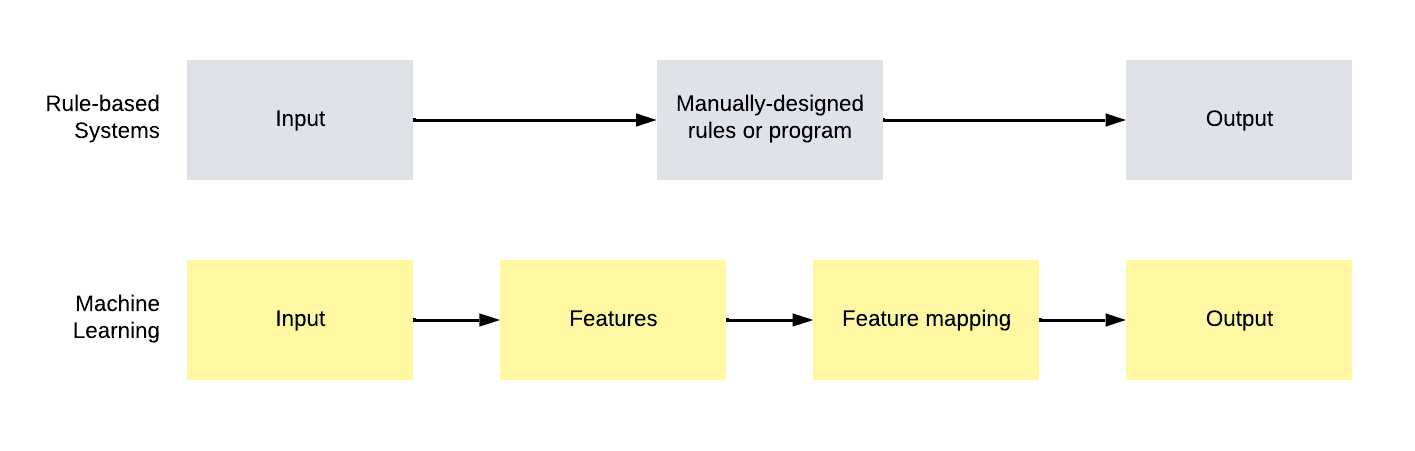
\includegraphics[width=\textwidth]{gambar/tipus_gambar_machine learning1}
	
	% Ubah dengan keterangan gambar yang diinginkan
	\caption{Perbandingan \emph{Machine Learning} dengan pemrograman biasa}
	\label{fig:machinelearning}
\end{figure}

\emph{Machine Learning} berbeda dengan pemrograman sistem tradisional yang berbasis peraturan. Seperti yang tertera pada Gambar 2.1, pemrograman tradisional memerlukan serangkaian peraturan atau program yang ditulis secara manual agar mendapatkan output yang diharapkan berdasarkan pada input yang dimasukkan. Sedangkan, pada \emph{machine learning}, tidak diperlukan untuk membuat program atau peraturannya secara manual, tapi bisa hanya dengan menentukan fitur-fitur data apa saja yang digunakan beserta hasil yang diinginkan. Secara otomatis, sistem akan mengoutputkan sebuah prediksi yang berdasarkan pada analisis dari data fitur dan algoritma statistika.

\subsection{Supervised Learning}
\label{sec:supervisedlearning}
Pada Supervised Learning, sistem akan menerima sejumlah contoh data yang telah dilabel untuk melakukan training dan membuat prediksi terhadap poin-poin yang belum terlihat. Metode ini paling sering ditemui pada permasalahan klasifikasi, regresi, dan ranking \citep{mohri2012foundations}. Supervised Learning dapat mengetahui suatu skenario dimana pada suatu contoh data training memiliki informasi signifikan yang tidak ada pada contoh data yang belum pernah dilihat. Dengan ini, maka diharapkan sistem dapat memprediksikan informasi yang tidak ada pada test data. Sistem ini dapat dianalogikan seperti seorang guru yang menjadi seorang supervisor terhadap muridnya dengan cara memberikan informasi tambahan, yaitu berupa label \citep{shalev2014understanding}.

\subsection{Unsupervised Learning}
\label{sec:unsupervisedlearning}
Pada Unsupervised Learning, sistem akan menerima sejumlah data tanpa label untuk melakukan training dan membuat prediksi terhadap poin-poin yang belum terlihat. Dikarenakan pada umumnya tidak ada contoh yang berlabel pada skenario tersebut maka akan lebih sulit untuk mengevaluasikan performa dari sistem secara kuantitatif. Contoh dari permasalahan Unsupervised Learning adalah seperti clustering dan dimensionality reduction \citep{mohri2012foundations}. Tidak ada perbedaan antara training dan test data pada unsupervised learning. SIstem akan memproses data input dengan tujuan untuk dapat mengambil suatu kesimpulan atau membuat kompresi dari data tersebut \citep{shalev2014understanding}.

\section{Deep Learning}
\label{sec:deeplearning}

Pada Gambar 2.2 tertera bahwa \emph{machine learning} merupakan suatu teknologi yang masih menjadi cakupan dari \emph{Artificial Intelligence} (AI). \emph{Deep learning} sendiri merupakan contoh dari \emph{representation learning}. Begitu pula dengan \emph{representation learning} merupakan contoh dari \emph{machine learning}. Teknologi seperti \emph{machine learning} dan \emph{representation learning} dinilai masih kurang mampu dalam menganalisis suatu data yang lebih kompleks dan memiliki sifat yang abstrak.

\begin{figure}[H]
	\centering
	
	% Ubah dengan nama file gambar dan ukuran yang akan digunakan
	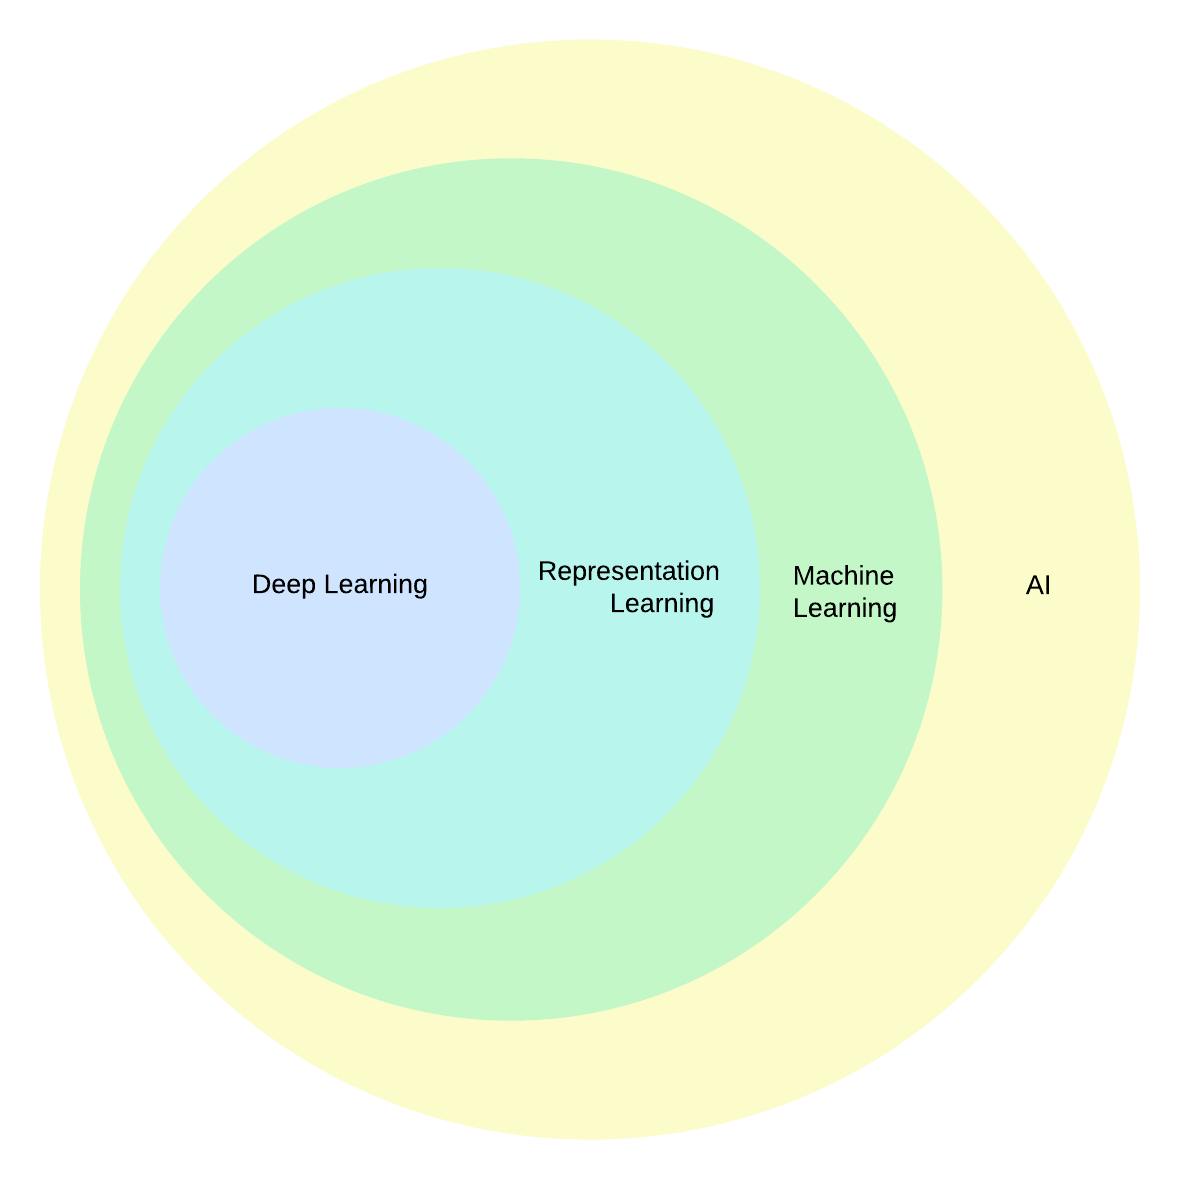
\includegraphics[width=0.8\textwidth]{gambar/tipus_gambar_deep learning venn}
	
	% Ubah dengan keterangan gambar yang diinginkan
	\caption{Diagram Venn teknologi \emph{Artificial Intelligence} (AI)}
	\label{fig:deeplearningvenn}
\end{figure}

Pada dunia pengaplikasian \emph{artificial intelligence} kesulitan yang sering dihadapi disebabkan oleh banyaknya variasi faktor-faktor yang mempengaruhi data yang sedang diobservasi. Sebagai contoh, tiap-tiap piksel dari sebuah gambar mobil berwarna merah akan lebih mendekati warna hitam pada malam hari. Selain itu, bentuk dari siluet mobil juga akan berubah-ubah bergantung pada sudut pandangnya. Umumnya, faktor-faktor variasi semacam ini perlu untuk diuraikan dan untuk variasi lain yang tidak diperlukan dapat diabaikan saja.

Tentunya, tidaklah mudah untuk mengekstrak fitur-fitur yang abstrak seperti yang disebutkan tadi melalui data mentahan. Contoh lainnya adalah seperti aksen dari seorang pembicara yang hanya dapat diidentifikasikan melalui kecerdasan yang mendekati kemampuan manusia dalam memahami hal tersebut. Deep Learning dapat menyeleaikan permasalahan seperti ini karena komputer dapat membangun suatu konsep yang kompleks dari hal yang sederhana. Salah satu contoh paling penting dari model \emph{deep learning} adalah seperti \emph{feed forward deep neutwork} atau \emph{multilayer perceptron} (MLP). \emph{Multilayer perceptron} adalah sebuah fungsi matematika yang memetakan nilai-nilai input ke output. Fungsi ini dibentuk dengan cara menggabungkan fungsi-fungsi yang lebih sederhana dan setiap fungsi ini akan memengaruhi hasil representasi dari input \citep{deepL}.

\begin{figure}[H]
	\centering
	
	% Ubah dengan nama file gambar dan ukuran yang akan digunakan
	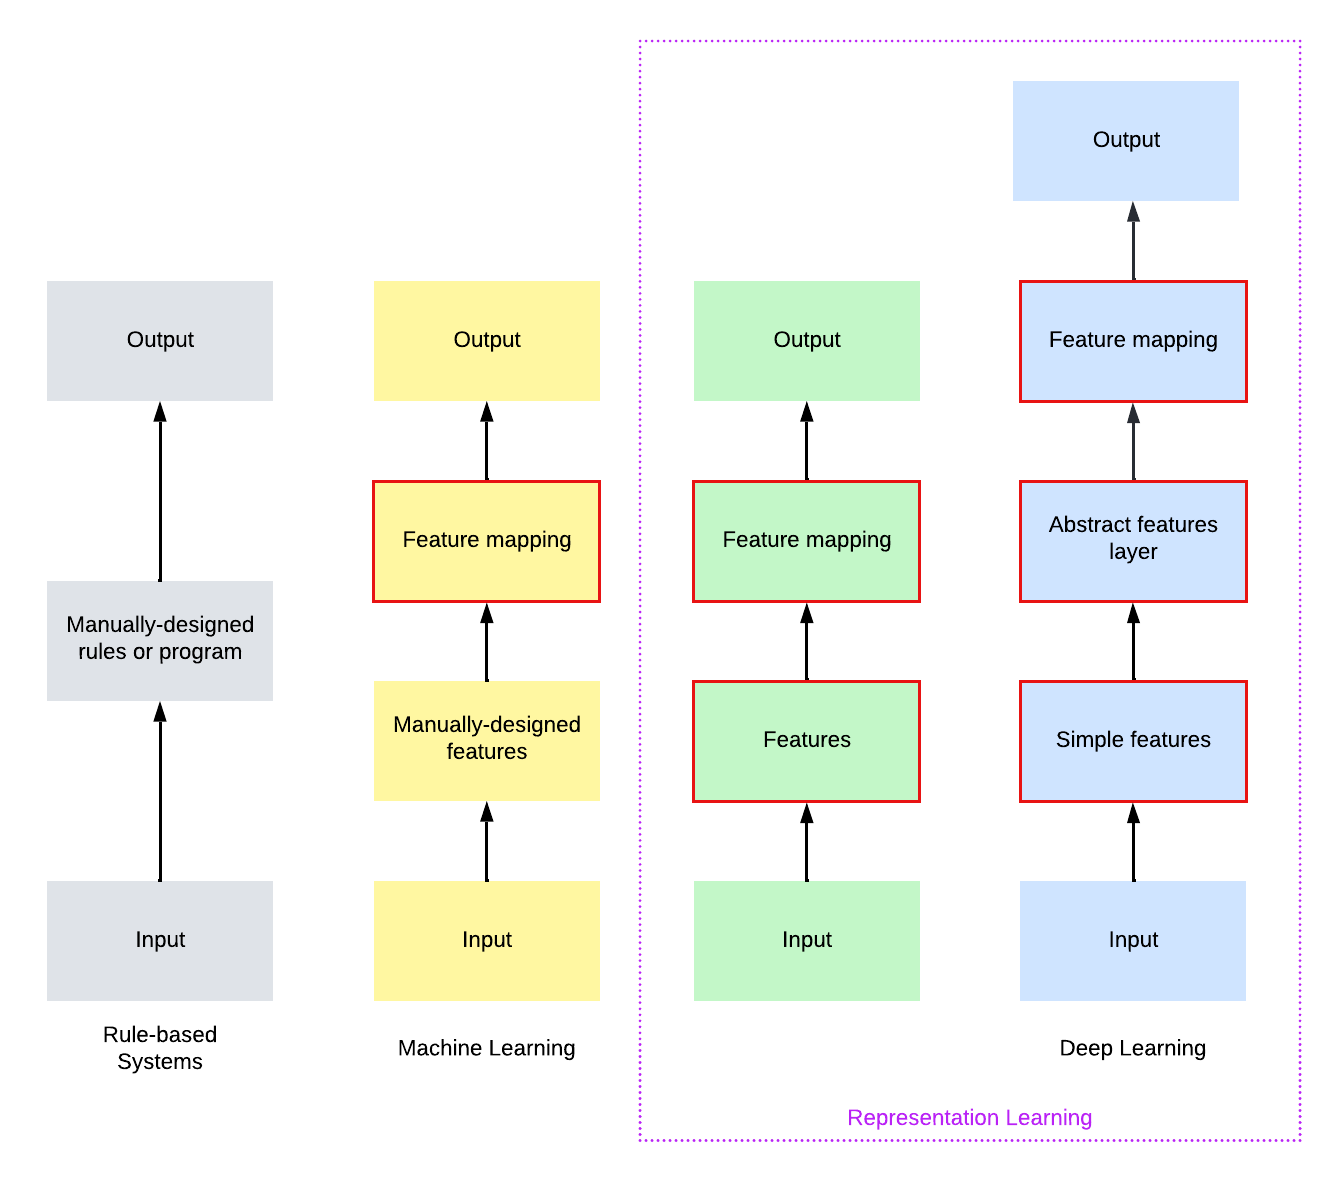
\includegraphics[width=0.8\textwidth]{gambar/tipus_gambar_deep learning}
	
	% Ubah dengan keterangan gambar yang diinginkan
	\caption{Perbandingan masing-masing teknologi \emph{machine learning} dan pemrograman biasa}
	\label{fig:deeplearningdiagram}
\end{figure}

Seperti yang telah dipaparkan pada Subbab 2.5 terlihat perbedaan dari \emph{machine learning} dengan pemrograman tradisional. Namun, masing-masing teknologi dari \emph{machine learning} sendiri memiliki beberapa perbedaan pula. Pada \emph{machine learning} klasik diperlukan fitur-fitur data yang didesain secara manual yang kemudian akan dilakukan pemetaan fitur. Kotak yang diberi \emph{outline} berwarna merah melambangkan bahwa komponen tersebut dapat dilakukan secara otomatis (dipelajari) oleh sistem. Berbeda dengan dengan \emph{representation learning} yang di mana sistem dapat memilih fitur-fitur yang diperlukan secara otomatis. Pada \emph{deep learning}, dibandingkan dengan \emph{representation learning}, hanya memerlukan fitur-fitur data simpel yang kemudian akan ditambahkan beberapa layer tambahan berisikan fitur-fitur yang lebih abstrak.

%Deep Learning merupakan salah satu pendekatan kecerdasan buatan dan tipe dari pembelajaran mesin. Deep Learning adalah salah satu jenis pembelajaran mesin yang dapat mencapai kekuatan yang tinggi serta fleksibilitas belajar untuk merepresentasikan dunia sebagai sebuah konsep nested hierarchy yang tiap-tiap konsepnya didefinisikan dalam kaitannya dengan konsep yang lebih sederhana, serta representasi yang lebih abstrak dikomputasikan dengan cara yang lebih tidak abstrak \citep{deepL}.

% input gambar
%\begin{figure} [H] \centering
% Nama dari file gambar yang diinputkan
%\includegraphics[scale=0.6]{gambar/umur.png}
% Keterangan gambar yang diinputkan
%\caption{Kategori umur menurut Depkes. RI (2009)}
% Label referensi dari gambar yang diinputkan
% \label{fig:Umur}
%\end{figure}

\section{Convolutional Neural Network (CNN)}
\label{sec:cnn}
Convolutional Neural Network adalah salah satu jenis dari neural network untuk memproses data yang memiliki topologi seperti grid. Contohnya adalah, data time-series yang dimana dapat digambarkan sebagai sebuah grid 1 dimensi yang mengambil sampel pada suatu interval waktu, dan data gambar yang dimana dapat dikatakan sebagai sebuah grid 2 dimensi berisikan piksel-piksel. Nama dari “Convolutional Neural Network” itu sendiri mengimplikasikan bahwa suatu network menggunakan operasi matematika yang disebut sebagai konvolusi. Konvolusi sendiri merupakan salah satu jenis dari operasi linear. Convolutional Network adalah sebuah neural network yang menggunakan konvolusi sebagai pengganti matriks perkalian umum di minimal salah satu lapisannya \citep{deepL}.

\section{\emph{Music Information Retrieval} (MIR)}
\label{sec:mir}

Music Information Retrieval (MIR) pertama diperkenalkan oleh Michael Kassler pada pertengahan dekade 1960-an. Perkembangan signifikan dari MIR ini diikuti oleh pertama kali didirikannya International Symposium on Music Information Retrieval (ISMIR) pada tahun 2000. Tujuan utama dari MIR adalah untuk memperbaiki akses penggemar musik terhadap koleksi musik dengan jumlah yang besar \citep{lefaivre2019characterizing}, terutama dengan berkembangnya platform-platform musik digital daring, jumlah pengguna maupun jumlah musik yang masuk ke dalam database juga makin besar sehingga diperlukan suatu sistem untuk mempermudah akses pengguna terhadap database musik tersebut. 

Penyimpanan dari musik sendiri dapat dibedakan menjadi dua kategori yang paling populer, yaitu continuous atau raw. Contoh dari formatnya adalah seperti MP3, wav, atau AIFF yang dimana juga menggambarkan kualitas dari audionya. Biasanya file-file tersebut disimpan dengan kualitas dan sample rate yang bermacam-macam. Contoh lain yang lebih jarang ditemui adalah pada format discrete, yaitu seperti MIDI, atau GUIDO. Format seperti ini biasanya secara digital dapat menggambarkan niatan dari si komposer meskipun biasanya format continuous memiliki jumlah data dan informasi yang jauh lebih banyak. Konversi antara kedua format biasanya hanya dapat dilakukan searah, yaitu dari discrete ke continuous \citep{McDermott2005TheSO}. 

\section{\emph{Mel-Frequency Coefficient of Cepstrum} (MFCC)}
\label{sec:mfcc}
%Mel-Frequency Cepstrum sangat efektif digunakan pada pengenalan suara, serta pemodelan subjective pitch dan konten frekuensi pada sinyal audio \citep{hmmaudio}.

Mel-Frequency Ceptral Coefficient (MFCC), dikembangkan oleh Davis dan Memelstein, merupakan sebuah metode ekstraksi fitur audio dengan cara menghitung koefisien ceptral berdasarkan variasi frekuensi kritis pada pendengaran manusia \citep{Widodo2017PenerapanMM}.
MFCC merepresentasikan sinyal pelafalan menjadi bentuk parametris untuk mempermudah pemrosesan dan analisis. Skala pitch yang memiliki jarak yang sama satu dengan lainnya disebut sebagai mel scale \citep{audiosignal1}.
MFCC merupakan fitur audio berbasis cepstrum yang paling sering digunakan. Hal ini dikarenakan MFCC dapat merepresentasikan vektor fitur dari sinyal musik maupun pelafalan, selain itu juga terbukti sangat berguna untuk klasifikasi audio pada umumnya \citep{li2019digital}.

\section{\emph{Confusion Matrix}}
\label{sec:confmatrix}

Confusion matrix adalah sebuah tabel yang merepresentasikan performa dari suatu model klasifikasi dalam memprediksi data ke berbagai macam class. Apabila sumbu x melambangkan prediction label maka sumbu y melambangkan true label-nya. Salah satu contohnya ada pada klasifikasi biner yang dimana hanya terdapat 2 class. Berikut seperti yang tertera pada Tabel 2.1 contoh dari tabel \emph{confusion matrix} untuk klasifikasi biner antara teks \emph{Spam} dan \emph{Not Spam}.

\begin{longtable}[c]{|c|c|c|}
	\caption{Contoh sederhana \emph{confusion matrix}}
	\label{tab:my-table}\\
	\hline
	& \textbf{Spam (predicted label)} & \textbf{Not Spam (predicted label)} \\ \hline
	\endfirsthead
	%
	\endhead
	%
	\textbf{Spam (true label)}     & 43 (TP)                         & 7 (FN)                              \\ \hline
	\textbf{Not Spam (true label)} & 11 (FP)                         & 39 (TN)                             \\ \hline
\end{longtable}

Seperti yang terlihat pada Tabel 2.1, terdapat 2 sumbu, yaitu kolom \emph{predicted label} dan baris \emph{true label}. \emph{True label} melambangkan label asli dari data, sedangkan \emph{predicted label} melambangkan label yang terprediksi oleh sistem. Dapat dilihat terdapat 43 data yang terprediksi dengan benar oleh sistem sebagai sebuah teks \emph{Spam}. Hal ini disebut sebagai \emph{True Positive} (TP). Selanjutnya terdapat pula data yang terprediksi sebagai sebuah \emph{Spam}, namun sebenarnya adalah \emph{Not Spam}, yaitu sebanyak 11 data. Hal ini disebut sebagai \emph{False Positive} (FP). Sebaliknya, juga terdapat data teks yang sebenarnya \emph{Not Spam} dan terprediksi oleh sistem dengan benar, yaitu sebanyak 39 data. Hal ini disebut sebagai \emph{True Negative} (TN). Terakhir, terdapat data yang terprediksi sebagai \emph{Not Spam} walaupun sebenarnya merupakan data teks \emph{Spam}, yaitu sebanyak 7 data. Hal ini disebut sebagai \emph{False Negative} (FN).
  \cleardoublepage

  % Bab 3 desain dan implementasi
  \chapter{METODOLOGI}
\label{chap:metodologi}

% Ubah bagian-bagian berikut dengan isi dari desain dan implementasi

\usetikzlibrary{positioning, fit, calc}   
\tikzset{block/.style={draw, thick, text width=2.5cm ,minimum height=1.3cm, align=center},   
	line/.style={-latex}     
}   

Penelitian ini dilaksanakan sesuai dengan desain sistem serta implementasinya. Desain sistem meliputi konsep serta langkah-langkah pembuatan dan perancangan infrastruktur yang digambarkan dalam bentuk blok-blok alur pengerjaan. Bagian implementasi berisikan pelaksanaan teknis untuk setiap blok pada desain sistem


\section{Peralatan}
\label{sec:peralatan}

Peralatan yang digunakan pada Tugas Akhir ini antara lain adalah Free Music Archive (FMA) Dataset, Google Colab, Anaconda Navigator, Visual Studio Code, Laptop, dan Desktop PC.

\subsection{Free Music Archive}
\label{subsec:fma}
Free Music Archive (FMA) merupakan sebuah dataset open-source yang biasa digunakan untuk keperluan Music Information Retrieval (MIR), seperti pengolahan data audio musik beserta fitur-fiturnya. Dataset ini berisikan 106.754 trek musik dengan metadatanya seperti ID, title, artist, genres, tags, dan play counts. Pada dataset ini terdapat total 161 genre (termasuk subgenre)\citep{fmadataset}.

\subsection{Anaconda Navigator}
\label{subsec:anacondanav}
Anaconda Navigator merupakan sebuah Graphical User Interface (GUI) untuk mendistribusikan Python dan R untuk segala keperluan komputasi ilmiah. Pada penelitian ini, Anaconda Navigator digunakan untuk men-deploy VS Code, serta instalasi segala package yang diperlukan.

\subsection{Visual Studio Code}
\label{subsec:vscode}
Visual Studio Code (VS Code) merupakan sebuah editor source code yang dikembangkan oleh Microsoft dan dapat digunakan untuk sistem operasi Windows, Linux, dan MacOS. Pada penelitian ini VS Code, disambungkan dengan Anaconda, digunakan untuk melakukan preprocessing serta training dataset.

\subsection{Desktop PC}
\label{subsec:desktop}
Desktop PC digunakan sebagai device untuk menjalankan Visual Studio Code dan penulisan buku. Berikut spesifikasi Desktop PC sesuai yang tertera pada Tabel 3.1.

\begin{table}[h]
	\centering
	
	\caption{Spesifikasi Desktop PC}
	\begin{adjustbox}{width=0.7\columnwidth, center}
	\begin{tabular}{|c|c|}
		\hline
		\textbf{Processor}        & Intel(R) Core(TM) i7-4790 CPU @ 3.60GHz \\ \hline
		\textbf{RAM}              & 16 GB DDR3                                \\ \hline
		\textbf{Storage}          & SSD 512 GB + HDD 1 TB                         \\ \hline
		\textbf{Graphics Card}    & AMD Radeon RX 5600 XT 6GB        \\ \hline
		\textbf{Operating System} & Windows 10 Home                           \\ \hline
	\end{tabular}
	\end{adjustbox}
	\label{fig:desktoptable}
\end{table}

\subsection{Laptop}
\label{subsec:laptop}

	Laptop digunakan untuk berbagai macam hal. Antara lain adalah sebagai device untuk menjalankan Visual Studio Code, melakukan training dataset, dan penulisan buku. Berikut spesifikasi laptop sesuai yang tertera pada Tabel 3.2.
	
	\begin{table}[h]
		\centering
		
		\caption{Spesifikasi Laptop}
		\begin{adjustbox}{width=0.7\columnwidth, center}
		\begin{tabular}{|c|c|}
			\hline
			\textbf{Processor}        & Intel(R) Core(TM) i5-10200H CPU @ 2.40GHz \\ \hline
			\textbf{RAM}              & 16 GB DDR4                                \\ \hline
			\textbf{Storage}          & SSD 512 GB + 1 TB                         \\ \hline
			\textbf{Graphics Card}    & Nvidia GeForce RTX 3060 6GB Laptop        \\ \hline
			\textbf{Operating System} & Windows 10 Home                           \\ \hline
		\end{tabular}
	\end{adjustbox}
		\label{fig:laptoptable}
	\end{table}

\section{Desain Sistem}
\label{sec:desainsistem}

Tugas Akhir ini mengimplementasikan Deep Learning untuk mengklasifikasikan subgenre dari suatu input potongan trek musik 30 detik yang berasal dari genre yang berbeda-beda menggunakan algoritma Convolutional Neural Network (CNN).

Tahapan sistem klasifikasi subgenre musik sesuai pada Gambar 3.1:

\begin{enumerate}
	\item Pengumpulan Data
	
	Dataset yang digunakan adalah Free Music Archive yang berisikan potongan-potongan musik dengan durasi 30 detik yang sudah dilabeli subgenrenya.
	\item Preprocessing Data
	
	Tahap ini meliputi pemotongan input trek menjadi beberapa segmen serta ekstraksi MFCC yang kemudian dikompilasikan di sebuah file json.
	\item Training
	
	Training dataset dilakukan pada model CNN yang telah dirancang.
	
	\item Testing
	
	Mengevaluasi model yang telah dilakukan training dengan simulasi test data yang kemudian dihitung akurasinya.
	
	\item Simulasi
	
	Setelah mendapatkan model yang optimal, sistem dapat digunakan untuk mengklasifikasikan suatu input musik ke dalam 3 subgenre yang paling masuk akal.
	
\end{enumerate}

\begin{figure}[b]
	\centering
	
	% Ubah dengan nama file gambar dan ukuran yang akan digunakan
	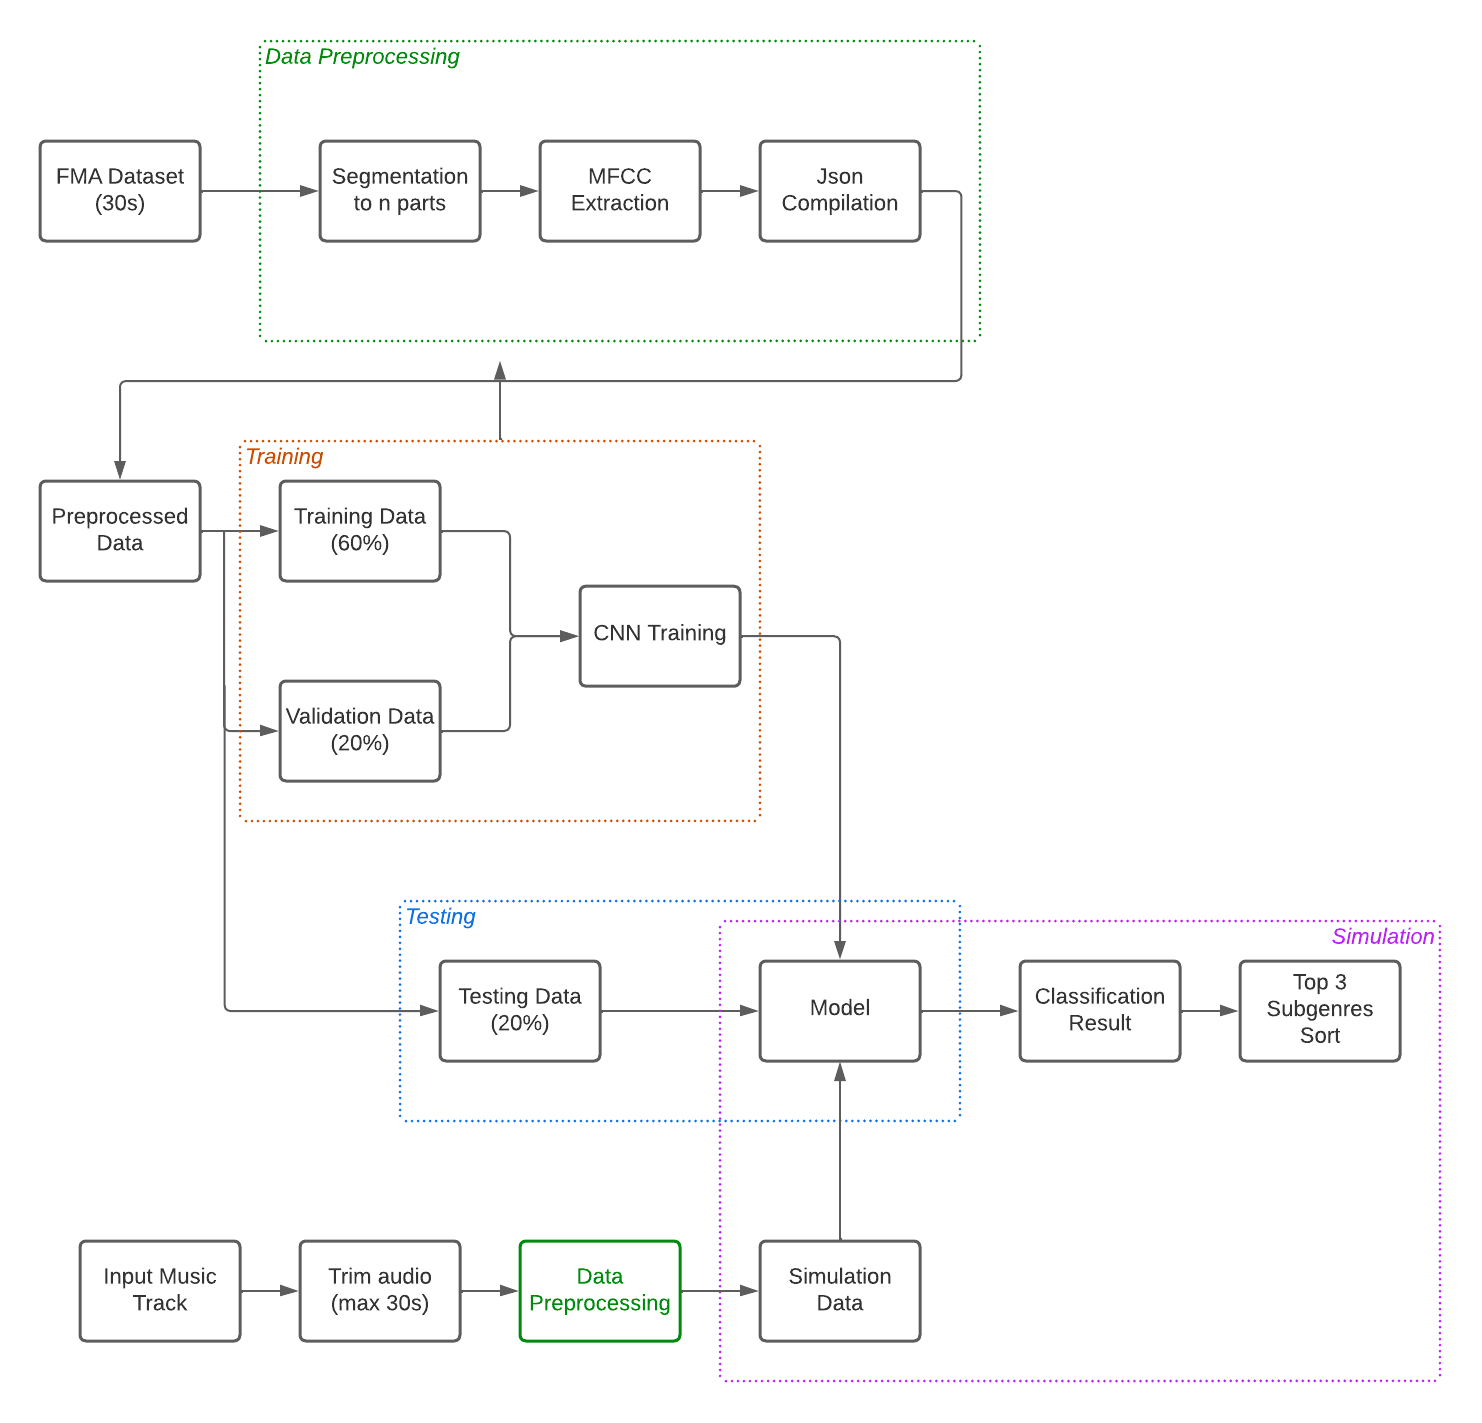
\includegraphics[width=\textwidth]{gambar/desain sistem2}
	
	% Ubah dengan keterangan gambar yang diinginkan
	\caption{Desain Sistem}
	\label{fig:desainsistem}
\end{figure}



\section{Pengumpulan Dataset}
\label{sec:pengumpulan dataset}

Dataset yang digunakan merupakan kumpulan musik dari 3 Genre, yaitu Rock, Folk, dan Electronic. Lalu, diambil masing-masing 3 Subgenre dengan jumlah trek sebanyak 200 tiap subgenrenya sehingga mencapai total 2700 trek. Kumpulan musik ini berupa file mp3 dari potongan 30 detik lagu yang disediakan oleh Free Music Archive(FMA) \citep{fmadataset}. FMA ini sendiri merupakan sebuah website yang berisikan kumpulan musik-musik royalty-free. Berikut tabel dataset yang digunakan pada Tugas Akhir ini:

\begin{table}[h]
	\centering
	
	\caption{Dataset yang digunakan}
	
	\begin{tabular}{|c|c|c|}
		\hline
		\textbf{Genre}              & \textbf{Subgenre} & \textbf{Jumlah} \\ \hline
		\multirow{3}{*}{Rock}       & Loud Rock         & 200             \\ \cline{2-3} 
		& Noise Rock        & 200             \\ \cline{2-3} 
		& Post Rock         & 200             \\ \hline
		\multirow{3}{*}{Folk}       & Freak Folk        & 200             \\ \cline{2-3} 
		& Free Folk         & 200             \\ \cline{2-3} 
		& Psych Folk        & 200             \\ \hline
		\multirow{3}{*}{Electronic} & Chiptune          & 200             \\ \cline{2-3} 
		& Glitch            & 200             \\ \cline{2-3} 
		& House             & 200             \\ \hline
	\end{tabular}
	
	\label{fig:dataset}
\end{table}

\section{Preprocessing Data}
\label{sec:preprocessing}

Sebelum dataset kumpulan musik diolah, perlu untuk dilakukan ekstraksi fitur yang dibutuhkan terlebih dahulu. Fitur yang digunakan pada Tugas Akhir ini adalah Mel-frequency cepstral coefficients (MFCC). Sebelum ekstraksi, dilakukan segmentasi file audio menjadi 10 segmen. Dengan ini, maka didapat potongan 3 detik sebanyak 10 buah per trek musik 30 detik. Hal ini dilakukan karena pada deep learning diperlukan jumlah dataset yang banyak. 

\begin{table}[h]
	
	\centering
	
	\caption{Parameter MFCC}
	
	\begin{tabular}{|l|l|}
		\hline
		\textbf{Parameter} & \textbf{Keterangan} \\ \hline
		Sample Rate        & 22050               \\ \hline
		N FFT              & 2048                \\ \hline
		Hop Length         & 512                 \\ \hline
		N MFCC             & 13                  \\ \hline
	\end{tabular}

	\label{fig:mfccparameter}
\end{table}

Setelah segmentasi, dilakukan ekstraksi MFCC dengan parameter seperti yang tertera pada Tabel 3.3. Berikut Gambar 3.2 adalah hasil contoh ekstraksi trek musik 30 detik menjadi 10 segmen MFCC.

\begin{figure}[h]
	\centering
	
	% Ubah dengan nama file gambar dan ukuran yang akan digunakan
	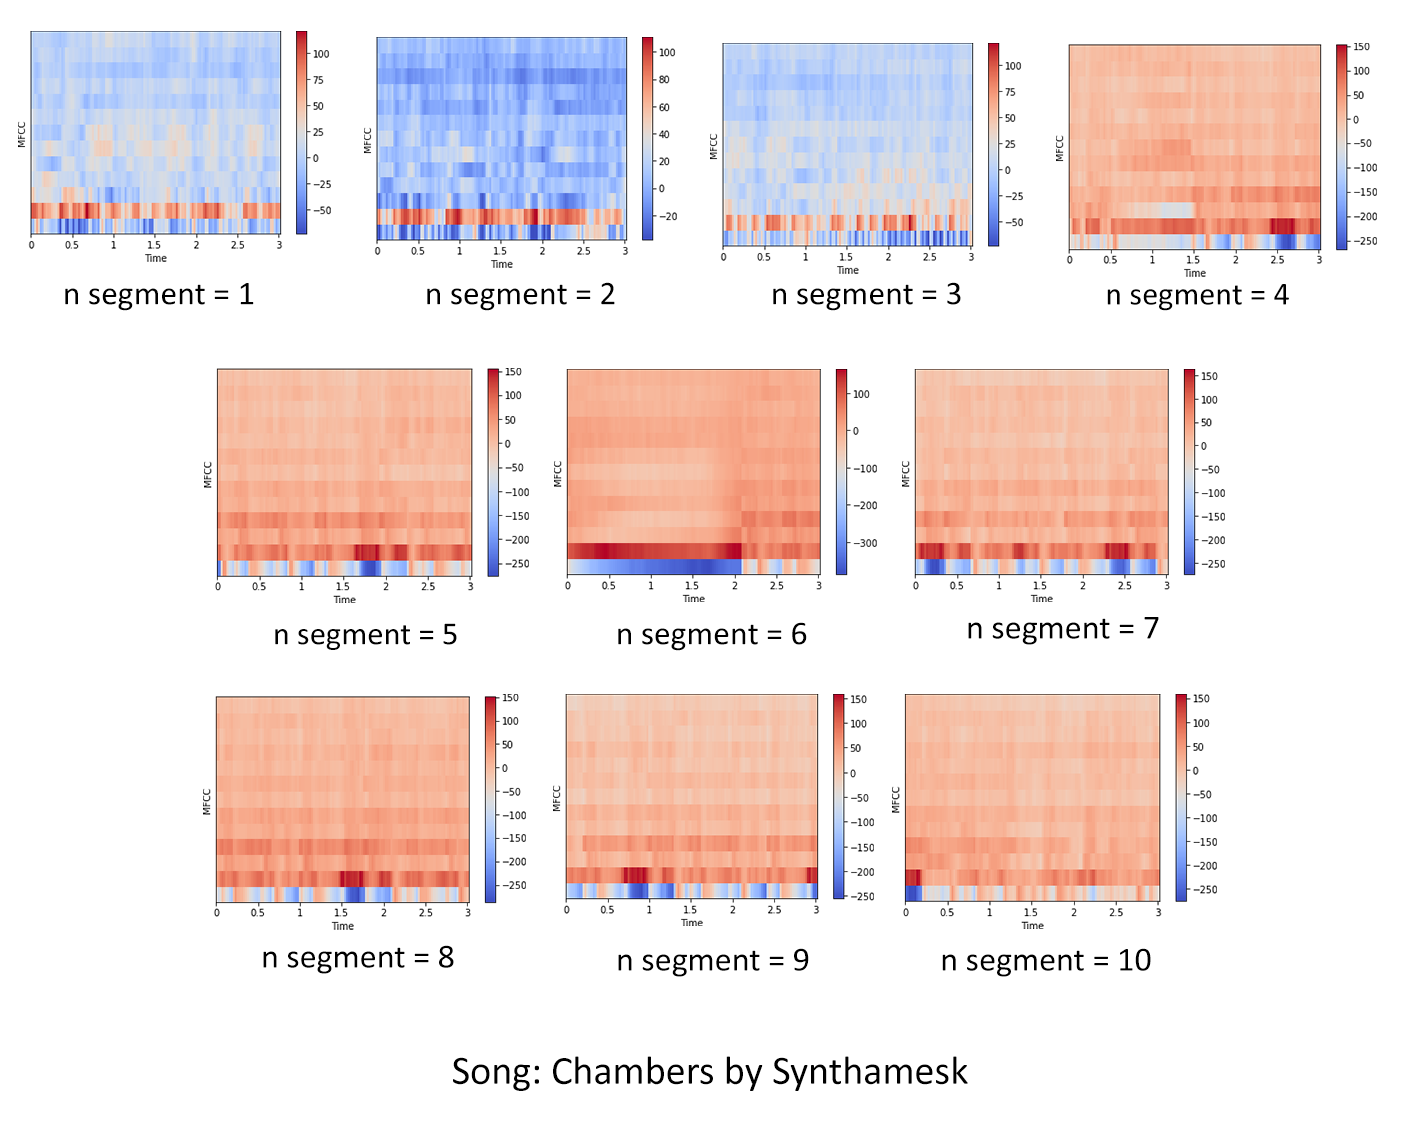
\includegraphics[width=\textwidth]{gambar/mfcc segments1}
	
	% Ubah dengan keterangan gambar yang diinginkan
	\caption{Plotting MFCC 10 Segmen}
	\label{fig:mfccsegmen}
\end{figure}

Ekstraksi dilakukan dengan menggunakan library dari python yang bernama LibROSA. Hasil ekstraksi MFCC tiap segmennya dilakukan transpose, kemudian dikompilasikan ke dalam sebuah file json. Pada file tersebut juga diberikan labeling untuk tiap subgenre (total 9 label) dan mapping untuk masing-masing label (0-8).

\section{Training}
\label{sec:training}

Setelah didapatkan hasil pemrosesan dataset serta pelabelannya, dilakukan training dataset agar komputer dapat mempelajari karakteristik dari masing-masing subgenre menggunakan fitur MFCC-nya. Dataset dibagi menjadi 3, yaitu Training Data (60\%), Validation Data (20\%), dan Test Data (20\%). Proses training dilakukan menggunakan framework Convolutional Neural Network (CNN). Layer disusun seperti yang tertera pada Tabel 3.5.

\begin{table}[h]
	\centering
	
	\caption{Susunan Layer CNN}
	
	\begin{tabular}{|l|l|l|}
		\hline
		\textbf{Layer (type)}                        & \textbf{Output Shape} & \textbf{Param \#} \\ \hline
		conv2d\_6 (Conv2D)                           & (None, 128, 11, 32)   & 320               \\ \hline
		max\_pooling2d\_6 (MaxPooling2D)             & (None, 64, 6, 32)     & 0                 \\ \hline
		batch\_normalization\_6 (BatchNormalization) & (None, 64, 6, 32)     & 128               \\ \hline
		activation\_6 (Activation)                   & (None, 64, 6, 32)     & 0                 \\ \hline
		dropout\_6 (Dropout)                         & (None, 64, 6, 32)     & 0                 \\ \hline
		conv2d\_7 (Conv2D)                           & (None, 62, 4, 64)     & 18496             \\ \hline
		max\_pooling2d\_7 (MaxPooling2D)             & (None, 31, 2, 64)     & 0                 \\ \hline
		batch\_normalization\_7 (BatchNormalization) & (None, 31, 2, 64)     & 256               \\ \hline
		activation\_7 (Activation)                   & (None, 31, 2, 64)     & 0                 \\ \hline
		dropout\_7 (Dropout)                         & (None, 31, 2, 64)     & 0                 \\ \hline
		conv2d\_8 (Conv2D)                           & (None, 30, 1, 32)     & 8224              \\ \hline
		max\_pooling2d\_8 (MaxPooling2D)             & (None, 15, 1, 32)     & 0                 \\ \hline
		batch\_normalization\_8 (BatchNormalization) & (None, 15, 1, 32)     & 128               \\ \hline
		activation\_8 (Activation)                   & (None, 15, 1, 32)     & 0                 \\ \hline
		flatten\_2 (Flatten)                         & (None, 480)           & 0                 \\ \hline
		dense\_4 (Dense)                             & (None, 64)            & 30784             \\ \hline
		dropout\_8 (Dropout)                         & (None, 64)            & 0                 \\ \hline
		dense\_5 (Dense)                             & (None, 9)             & 585               \\ \hline
	\end{tabular}

	\label{fig:layercnn}
\end{table}

Konfigurasi yang digunakan pada model dapat dilihat seusai seperti yang tertera pada Tabel 3.6.

\begin{table}[h]
	
	\centering
	
	\caption{Konfigurasi Model}
	
	\begin{tabular}{|l|l|}
		\hline
		\textbf{Jenis Konfigurasi} & \textbf{Keterangan} \\ \hline
		Classes                    & 9                   \\ \hline
		Batch                      & 8/16/32                 \\ \hline
		Epoch                      & 80/100                  \\ \hline
	\end{tabular}

	\label{fig:konfigurasimodel}
\end{table}

Classes merupakan jumlah label subgenre yang ingin diklasifikasikan. Batch size menentukan jumlah segmen MFCC yang diproses tiap Epoch-nya. Pada penelitian ini digunakan 3 Batch Size serta 2 Epoch yang berbeda untuk pengujian. 

\section{Testing}
\label{sec:testing}

Pada tahap testing, dilakukan perhitungan serta plotting confusion matrix untuk dapat melihat performa model untuk mengklasifikasikan masing-masing subgenre. Selain itu, dapat juga diketahui similaritas dari masing-masing subgenre serta hubungan antara satu dengan yang lainnya. Selanjutnya, dilakukan percobaan dengan input trek musik dengan berbagai macam durasi (maksimal 30 detik) dan melihat prediksi yang dilakukan oleh sistem dengan cara menampilkan 3 subgenre dengan probabilitas tertinggi.



  \cleardoublepage

  % Bab 4 pengujian dan analisis
  \chapter{HASIL DAN PEMBAHASAN}
\label{chap:hasilpembahasan}

% Ubah bagian-bagian berikut dengan isi dari hasil dan pembahasan

Pada penelitian ini dipaparkan hasil serta pembahasan mengenai pengujian dari desain sistem dan implementasi yang telah dilakukan. Pengujian dilakukan untuk mengetahui pengaruh dari \emph{batch size} dan \emph{epoch} pada akurasi training. Selain itu, pengujian durasi input audio simulasi dilaukan untuk mengetes pengaruh durasi terhadap performa akurasi dari sistem baik untuk masing-masing genre maupun secara keseluruhan.

\section{Hasil Training}
\label{sec:hasiltraining}
Berikut adalah hasil training untuk masing-masing parameter Batch Size dan Epoch sesuai yang tertera pada tahap pengujian:

\begin{figure}[H]
	\centering
	
	% Ubah dengan nama file gambar dan ukuran yang akan digunakan
	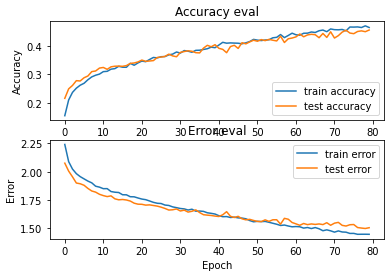
\includegraphics[width=0.6\textwidth]{gambar/b8_e80}
	
	% Ubah dengan keterangan gambar yang diinginkan
	\caption{Hasil Training Model Dengan Parameter Batch Size = 8, dan Epoch = 80}
	\label{fig:b8_e80}
\end{figure}

Seperti yang terlihat pada Gambar 4.1, pada Batch Size = 8, dan Epoch = 80 didapat nilai akurasi sebesar 45,33\%.

\begin{figure}[H]
	\centering
	
	% Ubah dengan nama file gambar dan ukuran yang akan digunakan
	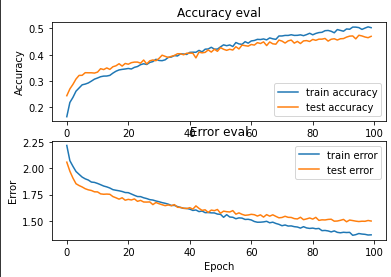
\includegraphics[width=0.6\textwidth]{gambar/b8_e100}
	
	% Ubah dengan keterangan gambar yang diinginkan
	\caption{Hasil Training Model Dengan Parameter Batch Size = 8, dan Epoch = 100}
	\label{fig:b8_e100}
\end{figure}

Seperti yang terlihat pada Gambar 4.2, pada Batch Size = 8, dan Epoch = 100 didapat nilai akurasi sebesar 47,69\%.

\begin{figure}[H]
	\centering
	
	% Ubah dengan nama file gambar dan ukuran yang akan digunakan
	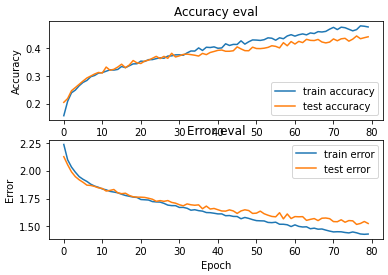
\includegraphics[width=0.6\textwidth]{gambar/b16_e80}
	
	% Ubah dengan keterangan gambar yang diinginkan
	\caption{Hasil Training Model Dengan Parameter Batch Size = 16, dan Epoch = 80}
	\label{fig:b16_e80}
\end{figure}

Seperti yang terlihat pada Gambar 4.3, pada Batch Size = 16, dan Epoch = 80 didapat nilai akurasi sebesar 44,39\%.

\begin{figure}[H]
	\centering
	
	% Ubah dengan nama file gambar dan ukuran yang akan digunakan
	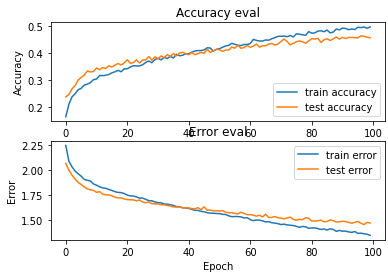
\includegraphics[width=0.6\textwidth]{gambar/b16_e100}
	
	% Ubah dengan keterangan gambar yang diinginkan
	\caption{Hasil Training Model Dengan Parameter Batch Size = 16, dan Epoch = 100}
	\label{fig:b16_e100}
\end{figure}

Seperti yang terlihat pada Gambar 4.4, pada Batch Size = 16, dan Epoch = 100 didapat nilai akurasi sebesar 47,21\%.

\begin{figure}[H]
	\centering
	
	% Ubah dengan nama file gambar dan ukuran yang akan digunakan
	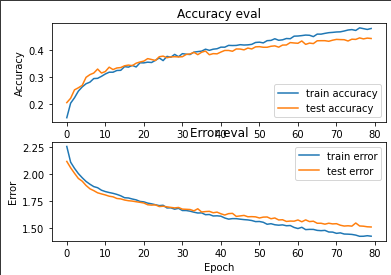
\includegraphics[width=0.6\textwidth]{gambar/b32_e80}
	
	% Ubah dengan keterangan gambar yang diinginkan
	\caption{Hasil Training Model Dengan Parameter Batch Size = 32, dan Epoch = 80}
	\label{fig:b32_e80}
\end{figure}

Seperti yang terlihat pada Gambar 4.5, pada Batch Size = 32, dan Epoch = 80 didapat nilai akurasi sebesar 45,07\%.

\begin{figure}[H]
	\centering
	
	% Ubah dengan nama file gambar dan ukuran yang akan digunakan
	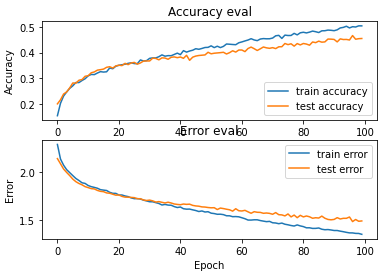
\includegraphics[width=0.6\textwidth]{gambar/b32_e100}
	
	% Ubah dengan keterangan gambar yang diinginkan
	\caption{Hasil Training Model Dengan Parameter Batch Size = 32, dan Epoch = 100}
	\label{fig:b32_e100}
\end{figure}

Seperti yang terlihat pada Gambar 4.6, pada Batch Size = 32, dan Epoch = 100 didapat nilai akurasi sebesar 46,39\%.

% Please add the following required packages to your document preamble:
% \usepackage{multirow}
% \usepackage{longtable}
% Note: It may be necessary to compile the document several times to get a multi-page table to line up properly
\begin{longtable}[c]{|c|c|c|}
	\caption{Tabel Hasil Akurasi pada Training}
	\label{tab:my-table}\\
	\hline
	\textbf{Epoch}       & \textbf{Batch Size} & \textbf{Akurasi (\%)} \\ \hline
	\endfirsthead
	%
	\endhead
	%
	\multirow{3}{*}{80}  & 8                   & 45,33                 \\ \cline{2-3} 
	& 16                  & 44,39                 \\ \cline{2-3} 
	& 32                  & 45,07                 \\ \hline
	\multirow{3}{*}{100} & 8                   & 47,69                 \\ \cline{2-3} 
	& 16                  & 47,21                 \\ \cline{2-3} 
	& 32                  & 46,39                 \\ \hline
\end{longtable}

Pada tahap ini dilakukan untuk melihat apabila dengan mengubah batch size dan epoch dapat mengubah akurasi model. Nilai akurasi dari masing-masing model telah dikompilasikan seperti yang tertera pada Tabel 4.1. Pada tabel tersebut dapat dilihat bahwa nilai batch size dan epoch telah mengubah akurasi model, namun tidak signifikan. Akurasi tertinggi didapat pada batch size = 8 dan epoch = 100 dengan nilai akurasi 47,69\%.

\section{Confusion Matrix}
\label{sec:confusionmatrix}
Confusion Matrix digunakan untuk melihat kualitas sistem dalam mengklasifikasikan subgenre dan untuk melihat similaritas dari masing-masing subgenrenya. Berikut yang tertera pada Gambar 4.7 hingga Gambar 4.12 adalah Confusion Matrix untuk masing-masing parameter \emph{Batch Size} dan \emph{Epoch} sesuai yang tertera pada rencana pengujian.

\begin{enumerate}
	\item Batch size = 8; Epoch = 80
	
	Seperti yang tertera pada Gambar 4.7 dapat diketahui bahwa subgenre Chiptune memiliki akurasi yang paling tinggi yaitu dengan skor 303. Sebaliknya, subgenre Psych Folk memiliki akurasi yang paling rendah yaitu dengan skor 152. Subgenre Chiptune paling sering salah diprediksikan sebagai genre Glitch dengan skor 37, Freak Folk paling sering salah diprediksikan sebagai Psych Folk dengan skor 53, Free Folk paling sering salah diprediksikan sebagai Glitch dan House dengan skor 74 dan 49, Glitch paling sering salah diprediksikan sebagai Post Rock dengan skor 45, House paling sering salah diprediksikan sebagai Glitch dan Free Folk dengan skor 56 dan 46, Loud Rock paling sering salah diprediksikan sebagai Noise Rock dan Post Rock dengan skor 68 dan 54, Noise Rock paling sering salah diprediksikan sebagai Post Rock dan Loud Rock dengan skor 41 dan 40, Post Rock paling sering salah diprediksikan sebagai Loud Rock dan Noise Rock dengan skor 34 dan 32, dan Psych Folk paling sering salah diprediksikan sebagai Post Rock dengan skor 48. 
	
	\begin{figure}[H]
		\centering
		
		% Ubah dengan nama file gambar dan ukuran yang akan digunakan
		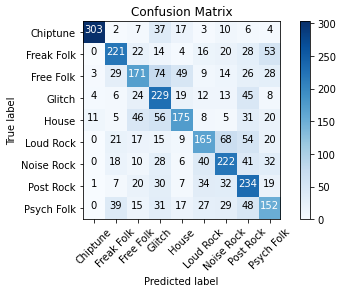
\includegraphics[width=0.8\textwidth]{gambar/confusion matrix_b8_e80}
		
		% Ubah dengan keterangan gambar yang diinginkan
		\caption{Confusion Matrix Model Dengan Parameter Batch Size = 8, dan Epoch = 80}
		\label{fig:cm_b8_e80}
	\end{figure}
	
	\item Batch size = 8; Epoch = 100
	
	Seperti yang tertera pada Gambar 4.8 dapat diketahui bahwa subgenre Chiptune memiliki akurasi yang paling tinggi yaitu dengan skor 289. Sebaliknya, subgenre Psych Folk memiliki akurasi yang paling rendah yaitu dengan skor 172. Subgenre Chiptune paling sering salah diprediksikan sebagai genre Glitch dengan skor 41, Freak Folk paling sering salah diprediksikan sebagai Post Rock dan Psych Folk dengan skor 38 dan 35, Free Folk paling sering salah diprediksikan sebagai House dengan skor 42, Glitch paling sering salah diprediksikan sebagai Post Rock dengan skor 35, House paling sering salah diprediksikan sebagai Free Folk 65, Loud Rock paling sering salah diprediksikan sebagai Post Rock dan Noise Rock dengan skor 53 dan 51, Noise Rock paling sering salah diprediksikan sebagai Post Rock dan Loud Rock dengan skor 58 dan 55, Post Rock paling sering salah diprediksikan sebagai Loud Rock dan Free Folk sama-sama dengan skor 23, dan Psych Folk paling sering salah diprediksikan sebagai Post Rock dengan skor 57.
	
	\begin{figure}[H]
		\centering
		
		% Ubah dengan nama file gambar dan ukuran yang akan digunakan
		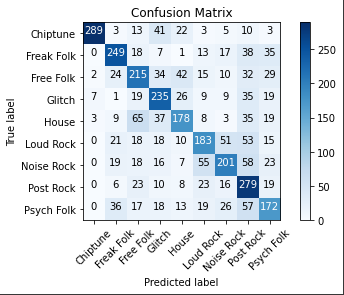
\includegraphics[width=0.8\textwidth]{gambar/confusion matrix_b8_e100}
		
		% Ubah dengan keterangan gambar yang diinginkan
		\caption{Confusion Matrix Model Dengan Parameter Batch Size = 8, dan Epoch = 100}
		\label{fig:cm_b8_e100}
	\end{figure}

	\item Batch size = 16; Epoch = 80
	
	Seperti yang tertera pada Gambar 4.9 dapat diketahui bahwa subgenre Chiptune memiliki akurasi yang paling tinggi yaitu dengan skor 290. Sebaliknya, subgenre House memiliki akurasi yang paling rendah yaitu dengan skor 141. Subgenre Chiptune paling sering salah diprediksikan sebagai genre Glitch dengan skor 40, Freak Folk paling sering salah diprediksikan sebagai Psych Folk dengan skor 73, Free Folk paling sering salah diprediksikan sebagai Glitch dan House dengan skor 59 dan 44, Glitch paling sering salah diprediksikan sebagai Post Rock dengan skor 39, House paling sering salah diprediksikan sebagai Glitch dan Free Folk dengan skor 65 dan 59, Loud Rock paling sering salah diprediksikan sebagai Noise Rock dan Post Rock dengan skor 78 dan 67, Noise Rock paling sering salah diprediksikan sebagai Loud Rock dan Post Rock dengan skor 36 dan 35, Post Rock paling sering salah diprediksikan sebagai Noise Rock dan Psych Folk sama-sama dengan skor, dan Psych Folk paling sering salah diprediksikan sebagai Post Rock dengan skor 51.
	
	\begin{figure}[H]
		\centering
		
		% Ubah dengan nama file gambar dan ukuran yang akan digunakan
		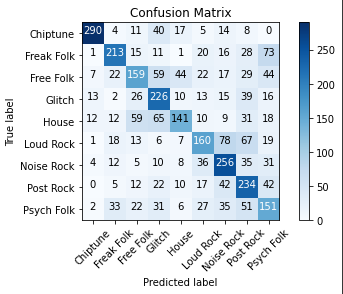
\includegraphics[width=0.8\textwidth]{gambar/confusion matrix_b16_e80}
		
		% Ubah dengan keterangan gambar yang diinginkan
		\caption{Confusion Matrix Model Dengan Parameter Batch Size = 16, dan Epoch = 80}
		\label{fig:cm_b16_e80}
	\end{figure}

	\item Batch size = 16; Epoch = 100
	
	Seperti yang tertera pada Gambar 4.10 dapat diketahui bahwa subgenre Chiptune memiliki akurasi yang paling tinggi yaitu dengan skor 302. Sebaliknya, subgenre Psych Folk memiliki akurasi yang paling rendah yaitu dengan skor 151. Subgenre Chiptune paling sering salah diprediksikan sebagai genre Glitch dengan skor 31, Freak Folk paling sering salah diprediksikan sebagai Post Rock dengan skor 35, Free Folk paling sering salah diprediksikan sebagai Post Rock dan House dengan skor 43 dan 42, Glitch paling sering salah diprediksikan sebagai Post Rock dengan skor 37, House paling sering salah diprediksikan sebagai Free Folk dan Glitch dengan skor 57 dan 53, Loud Rock paling sering salah diprediksikan sebagai Noise Rock dan Post Rock dengan skor 68 dan 50, Noise Rock paling sering salah diprediksikan sebagai Loud Rock dan Post Rock dengan skor 58 dan 48, Post Rock paling sering salah diprediksikan sebagai Noise Rock dengan skor 48, dan Psych Folk paling sering salah diprediksikan sebagai Freak Folk dan Post Rock dengan skor 55 dan 48.
	
	\begin{figure}[H]
		\centering
		
		% Ubah dengan nama file gambar dan ukuran yang akan digunakan
		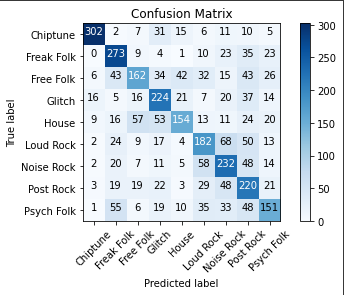
\includegraphics[width=0.8\textwidth]{gambar/confusion matrix_b16_e100}
		
		% Ubah dengan keterangan gambar yang diinginkan
		\caption{Confusion Matrix Model Dengan Parameter Batch Size = 16, dan Epoch = 100}
		\label{fig:cm_b16_e100}
	\end{figure}

	\item Batch size = 32; Epoch = 80
	
	Seperti yang tertera pada Gambar 4.11 dapat diketahui bahwa subgenre Chiptune memiliki akurasi yang paling tinggi yaitu dengan skor 299. Sebaliknya, subgenre Free Folk memiliki akurasi yang paling rendah yaitu dengan skor 139. Subgenre Chiptune paling sering salah diprediksikan sebagai genre Glitch dengan skor 26, Freak Folk paling sering salah diprediksikan sebagai Psych Folk dengan skor 41, Free Folk paling sering salah diprediksikan sebagai House dan Glitch dengan skor 65 dan 53, Glitch paling sering salah diprediksikan sebagai Post Rock dengan skor 38, House paling sering salah diprediksikan sebagai Glitch dengan skor 51, Loud Rock paling sering salah diprediksikan sebagai Noise Rock dan Post Rock dengan skor 55 dan 48, Noise Rock paling sering salah diprediksikan sebagai Loud Rock dengan skor 74, Post Rock paling sering salah diprediksikan sebagai Psych Folk dengan skor 56, dan Psych Folk paling sering salah diprediksikan sebagai Freak Folk dan Loud Rock dengan skor 50 dan 48.
	
	\begin{figure}[H]
		\centering
		
		% Ubah dengan nama file gambar dan ukuran yang akan digunakan
		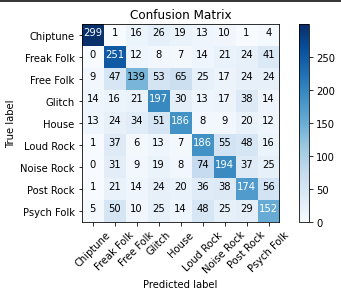
\includegraphics[width=0.8\textwidth]{gambar/confusion matrix_b32_e80}
		
		% Ubah dengan keterangan gambar yang diinginkan
		\caption{Confusion Matrix Model Dengan Parameter Batch Size = 32, dan Epoch = 80}
		\label{fig:cm_b32_e80}
	\end{figure}

	\item Batch size = 32; Epoch = 100
	
	Seperti yang tertera pada Gambar 4.12 dapat diketahui bahwa subgenre Chiptune memiliki akurasi yang paling tinggi yaitu dengan skor 275. Sebaliknya, subgenre Psych Folk memiliki akurasi yang paling rendah yaitu dengan skor 133. Subgenre Chiptune paling sering salah diprediksikan sebagai House dan Glitch dengan skor 37 dan 35, Freak Folk paling sering salah diprediksikan sebagai Free Folk dan Psych Folk dengan skor 29 dan 27, Free Folk paling sering salah diprediksikan sebagai House dan Glitch dengan skor 61 dan 48, Glitch paling sering salah diprediksikan sebagai Free Folk dengan skor 39, House paling sering salah diprediksikan sebagai Glitch dan Free Folk dengan skor 56 dan 48, Loud Rock paling sering salah diprediksikan sebagai Noise Rock dengan skor 73, Noise Rock paling sering salah diprediksikan sebagai Loud Rock dengan skor 67, Post Rock paling sering salah diprediksikan sebagai Noise Rock dan Loud Rock dengan skor 57 dan 45, dan Psych Folk paling sering salah diprediksikan sebagai Freak Folk dengan skor 59.
	
	\begin{figure}[H]
		\centering
		
		% Ubah dengan nama file gambar dan ukuran yang akan digunakan
		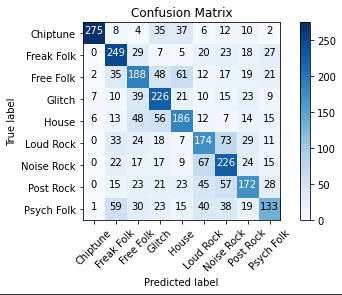
\includegraphics[width=0.8\textwidth]{gambar/confusion matrix_b32_e100}
		
		% Ubah dengan keterangan gambar yang diinginkan
		\caption{Confusion Matrix Model Dengan Parameter Batch Size = 32, dan Epoch = 100}
		\label{fig:cm_b32_e100}
	\end{figure}

\end{enumerate}

Dari hasil yang didapat diatas dapat dikatakan bahwa sistem dapat mengklasifikasikan subgenre Chiptune dengan baik, namun sebaliknya pengklasifikasian subgenre Psych Folk masih sering disalah artikan sebagai subgenre lainnya, seperti Post Rock, Loud Rock, Noise Rock, dan Freak Folk.

\section{Analisis Simulasi}
\label{sec:analisissimulasi}

Tahap simulasi ini dilakukan untuk mencari tahu bagaimana performa dari sistem pada data-data baru yang sudah diberi \emph{true label}. Kemudian, dilakukan analisis untuk hasilnya pada masing-masing genre dan keseluruhannya.

\subsection{Dataset Simulasi}
\label{subsec:datasetsimulasi}

Dataset simulasi yang digunakan, sama seperti dataset training, merupakan kumpulan musik dari 3 Genre, yaitu Rock, Folk, dan Electronic. Lalu, diambil masing-masing 3 Subgenre dengan jumlah trek sebanyak 100 tiap subgenrenya sehingga mencapai total 900 trek. Kumpulan musik ini berupa file mp3 dari potongan 30 detik lagu yang disediakan oleh \emph{Free Music Archive} (FMA) \citep{DBLP:journals/corr/BenziDVB16} yang kemudian dilakukan proses pemotongan durasi menjadi 3, 9, 15, dan 30 detik. Dari sini maka didapat total potongan lagu sebanyak 3600 trek yang berisikan 900 trek pada masing-masing durasinya. Berikut tabel dataset yang digunakan untuk simulasi ini tertera pada Tabel 4.1.

\begin{longtable}[c]{|c|c|c|}
	\caption{Dataset simulasi yang digunakan}
	\label{tab:my-table}\\
	\hline
	\textbf{Genre}              & \textbf{Subgenre} & \textbf{Jumlah} \\ \hline
	\endfirsthead
	%
	\endhead
	%
	\multirow{3}{*}{Rock}       & Loud Rock         & 100             \\ \cline{2-3} 
	& Noise Rock        & 100             \\ \cline{2-3} 
	& Post Rock         & 100             \\ \hline
	\multirow{3}{*}{Folk}       & Freak Folk        & 100             \\ \cline{2-3} 
	& Free Folk         & 100             \\ \cline{2-3} 
	& Psych Folk        & 100             \\ \hline
	\multirow{3}{*}{Electronic} & Chiptune          & 100             \\ \cline{2-3} 
	& Glitch            & 100             \\ \cline{2-3} 
	& House             & 100             \\ \hline
\end{longtable}

\subsection{Contoh Hasil Klasifikasi}
\label{subsec:contohklasifikasi}

Seperti yang telah dipaparkan pada Desain Sistem, untuk hasil pengklasifikasiannya menampilkan 3 subgenre tertinggi yang paling masuk akal beserta dengan persentasenya. Berikut contoh output dari simulasi yang telah dilakukan masing-masing 1 trek untuk tiap subgenre dapat dilihat pada Gambar 4.13 hingga Gambar 4.21. Penulisan dari yang tertinggi berurutan dari kiri ke kanan.

\begin{enumerate}
	\item Chiptune
	
	\begin{figure}[H]
		\centering
		
		% Ubah dengan nama file gambar dan ukuran yang akan digunakan
		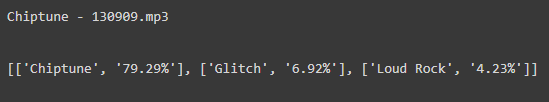
\includegraphics[width=0.8\textwidth]{gambar/classification_chiptune}
		
		% Ubah dengan keterangan gambar yang diinginkan
		\caption{Hasil Klasifikasi Subgenre Chiptune}
		\label{fig:klas_chiptune}
	\end{figure}
	
	Pada Gambar 4.13 dapat dilihat bahwa pada file bernama 130909.mp3 \emph{true label} subgenrenya, yaitu Chiptune, mendapati urutan ke pertama dengan persentase prediksinya yaitu 79,29\% yang diikuti oleh Glitch dengan persentasenya 6,92\% dan Loud Rock dengan persentasenya 4,23\%.
	
	\item Glitch
	
	\begin{figure}[H]
		\centering
		
		% Ubah dengan nama file gambar dan ukuran yang akan digunakan
		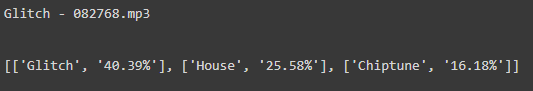
\includegraphics[width=0.8\textwidth]{gambar/classification_glitch}
		
		% Ubah dengan keterangan gambar yang diinginkan
		\caption{Hasil Klasifikasi Subgenre Glitch}
		\label{fig:klas_glitch}
	\end{figure}
	
	Pada Gambar 4.14 dapat dilihat bahwa pada file bernama 082768.mp3 \emph{true label} Glitch, yaitu Glitch, mendapati urutan ke pertama dengan persentase prediksinya yaitu 40,39\% yang diikuti oleh House dengan persentasenya 25,58\% dan Chiptune dengan persentasenya 16,18\%.
	
	\item House
	
	\begin{figure}[H]
		\centering
		
		% Ubah dengan nama file gambar dan ukuran yang akan digunakan
		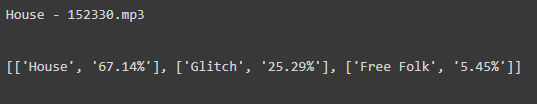
\includegraphics[width=0.8\textwidth]{gambar/classification_house}
		
		% Ubah dengan keterangan gambar yang diinginkan
		\caption{Hasil Klasifikasi Subgenre House}
		\label{fig:klas_house}
	\end{figure}
	
	Pada Gambar 4.15 dapat dilihat bahwa pada file bernama 152330.mp3 \emph{true label} subgenrenya, yaitu House, mendapati urutan ke pertama dengan persentase prediksinya yaitu 67,14\% yang diikuti oleh Glitch dengan persentasenya 25,29\% dan Free Folk dengan persentasenya 5,45\%.
	
	\item Freak Folk
	
	\begin{figure}[H]
		\centering
		
		% Ubah dengan nama file gambar dan ukuran yang akan digunakan
		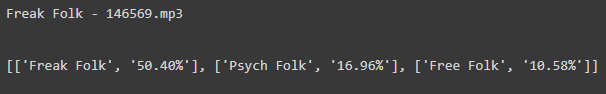
\includegraphics[width=0.8\textwidth]{gambar/classification_freak folk}
		
		% Ubah dengan keterangan gambar yang diinginkan
		\caption{Hasil Klasifikasi Subgenre Freak Folk}
		\label{fig:klas_freakfolk}
	\end{figure}
	
	Pada Gambar 4.16 dapat dilihat bahwa pada file bernama 146569.mp3 \emph{true label} subgenrenya, yaitu Freak Folk, mendapati urutan ke pertama dengan persentase prediksinya yaitu 50,40\% yang diikuti oleh Psych Folk dengan persentasenya 16,96\% dan Free Folk dengan persentasenya 10,58\%.
	
	\item Free Folk
	
	\begin{figure}[H]
		\centering
		
		% Ubah dengan nama file gambar dan ukuran yang akan digunakan
		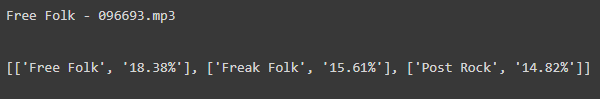
\includegraphics[width=0.8\textwidth]{gambar/classification_free folk}
		
		% Ubah dengan keterangan gambar yang diinginkan
		\caption{Hasil Klasifikasi Subgenre Free Folk}
		\label{fig:klas_freefolk}
	\end{figure}
	
	Pada Gambar 4.17 dapat dilihat bahwa pada file bernama 096693.mp3 \emph{true label} subgenrenya, yaitu Free Folk, mendapati urutan ke pertama dengan persentase prediksinya yaitu 18,38\% yang diikuti oleh Freak Folk dengan persentasenya 15,61\% dan Post Rock dengan persentasenya 14,82\%.
	
	\item Psych Folk
	
	\begin{figure}[H]
		\centering
		
		% Ubah dengan nama file gambar dan ukuran yang akan digunakan
		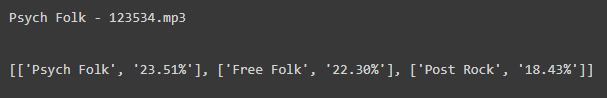
\includegraphics[width=0.8\textwidth]{gambar/classification_psych folk}
		
		% Ubah dengan keterangan gambar yang diinginkan
		\caption{Hasil Klasifikasi Subgenre Psych Folk}
		\label{fig:klas_psychfolk}
	\end{figure}
	
	Pada Gambar 4.18 dapat dilihat bahwa pada file bernama 123534.mp3 \emph{true label} subgenrenya, yaitu Psych Folk, mendapati urutan ke pertama dengan persentase prediksinya yaitu 23,51\% yang diikuti oleh Free Folk dengan persentasenya 22,30\% dan Post Rock dengan persentasenya 18,43\%.
	
	\item Loud Rock
	
	\begin{figure}[H]
		\centering
		
		% Ubah dengan nama file gambar dan ukuran yang akan digunakan
		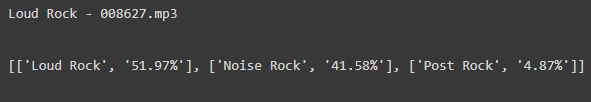
\includegraphics[width=0.8\textwidth]{gambar/classification_loud rock}
		
		% Ubah dengan keterangan gambar yang diinginkan
		\caption{Hasil Klasifikasi Subgenre Loud Rock}
		\label{fig:klas_loudrock}
	\end{figure}
	
	Pada Gambar 4.19 dapat dilihat bahwa pada file bernama 008627.mp3 \emph{true label} subgenrenya, yaitu Loud Rock, mendapati urutan ke pertama dengan persentase prediksinya yaitu 51,97\% yang diikuti oleh Noise Rock dengan persentasenya 41,58\% dan Post Rock dengan persentasenya 4,87\%.
	
	\item Noise Rock
	
	\begin{figure}[H]
		\centering
		
		% Ubah dengan nama file gambar dan ukuran yang akan digunakan
		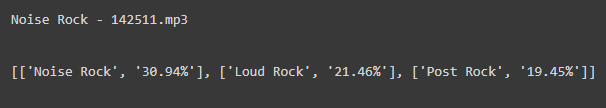
\includegraphics[width=0.8\textwidth]{gambar/classification_noise rock}
		
		% Ubah dengan keterangan gambar yang diinginkan
		\caption{Hasil Klasifikasi Subgenre Noise Rock}
		\label{fig:klas_noiserock}
	\end{figure}
	
	Pada Gambar 4.20 dapat dilihat bahwa pada file bernama 142511.mp3 \emph{true label} subgenrenya, yaitu Noise Rock, mendapati urutan ke pertama dengan persentase prediksinya yaitu 30,94\% yang diikuti oleh Loud Rock dengan persentasenya 21,46\% dan Post Rock dengan persentasenya 19,45\%.
	
	\item Post Rock
	
	\begin{figure}[H]
		\centering
		
		% Ubah dengan nama file gambar dan ukuran yang akan digunakan
		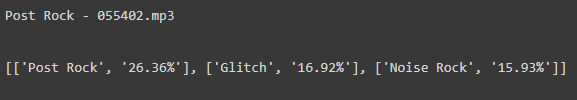
\includegraphics[width=0.8\textwidth]{gambar/classification_post rock}
		
		% Ubah dengan keterangan gambar yang diinginkan
		\caption{Hasil Klasifikasi Subgenre Post Rock}
		\label{fig:klas_postrock}
	\end{figure}
	
	Pada Gambar 4.21 dapat dilihat bahwa pada file bernama 055402.mp3 \emph{true label} subgenrenya, yaitu Post Rock, mendapati urutan ke pertama dengan persentase prediksinya yaitu 26,36\% yang diikuti oleh Glitch dengan persentasenya 16,92\% dan Noise Rock dengan persentasenya 15,93\%.
	
\end{enumerate}

\subsection{Hasil Simulasi}
\label{subsec:hasilsimulasi}

Berikut merupakan penggambaran dari hasil simulasi dalam bentuk tabel menggunakan dataset simulasi yang telah dilakukan pada penelitian dapat dilihat pada Tabel 4.2 hingga Tabel 4.25.

\begin{longtable}[c]{|c|c|c|c|c|}
	\hline
	\textbf{}      & \textbf{1st} & \textbf{2nd} & \textbf{3rd} & \textbf{None} \\ \hline
	\endfirsthead
	%
	\endhead
	%
	Chiptune       & 53           & 11           & 6            & 30            \\ \hline
	Glitch         & 41           & 21           & 8            & 30            \\ \hline
	House          & 33           & 24           & 15           & 28            \\ \hline
	Freak Folk     & 42           & 15           & 5            & 38            \\ \hline
	Free Folk      & 28           & 25           & 21           & 26            \\ \hline
	Psych Folk     & 23           & 21           & 11           & 45            \\ \hline
	Loud Rock      & 29           & 22           & 8            & 41            \\ \hline
	Noise Rock     & 33           & 17           & 12           & 38            \\ \hline
	Post Rock      & 33           & 12           & 20           & 35            \\ \hline
	\textbf{Total} & \textbf{315} & \textbf{168} & \textbf{106} & \textbf{311}  \\ \hline
	\caption{Tabel Hasil Simulasi dengan Batch Size = 8, Epoch = 80, dan Durasi = 3 detik}
	\label{tab:my-table}\\
\end{longtable}

\begin{longtable}[c]{|c|c|c|c|c|}
	\hline
	\textbf{}      & \textbf{1st} & \textbf{2nd} & \textbf{3rd} & \textbf{None} \\ \hline
	\endfirsthead
	%
	\endhead
	%
	Chiptune       & 64           & 7            & 6            & 23            \\ \hline
	Glitch         & 43           & 19           & 11           & 27            \\ \hline
	House          & 39           & 19           & 14           & 28            \\ \hline
	Freak Folk     & 50           & 14           & 9            & 27            \\ \hline
	Free Folk      & 33           & 19           & 20           & 28            \\ \hline
	Psych Folk     & 27           & 19           & 12           & 42            \\ \hline
	Loud Rock      & 27           & 26           & 7            & 40            \\ \hline
	Noise Rock     & 34           & 23           & 10           & 33            \\ \hline
	Post Rock      & 30           & 14           & 17           & 39            \\ \hline
	\textbf{Total} & \textbf{347} & \textbf{160} & \textbf{106} & \textbf{287}  \\ \hline
	\caption{Tabel Hasil Simulasi dengan Batch Size = 8, Epoch = 80, dan Durasi = 9 detik}
	\label{tab:my-table}\\
\end{longtable}

\begin{longtable}[c]{|c|c|c|c|c|}
	\hline
	\textbf{}      & \textbf{1st} & \textbf{2nd} & \textbf{3rd} & \textbf{None} \\ \hline
	\endfirsthead
	%
	\endhead
	%
	Chiptune       & 63           & 7            & 10           & 20            \\ \hline
	Glitch         & 48           & 18           & 10           & 24            \\ \hline
	House          & 35           & 24           & 16           & 25            \\ \hline
	Freak Folk     & 48           & 14           & 10           & 28            \\ \hline
	Free Folk      & 30           & 26           & 19           & 25            \\ \hline
	Psych Folk     & 25           & 22           & 16           & 37            \\ \hline
	Loud Rock      & 28           & 25           & 9            & 38            \\ \hline
	Noise Rock     & 35           & 24           & 9            & 32            \\ \hline
	Post Rock      & 33           & 11           & 16           & 40            \\ \hline
	\textbf{Total} & \textbf{345} & \textbf{171} & \textbf{115} & \textbf{269}  \\ \hline
	\caption{Tabel Hasil Simulasi dengan Batch Size = 8, Epoch = 80, dan Durasi = 15 detik}
	\label{tab:my-table}\\
\end{longtable}

% Please add the following required packages to your document preamble:
% \usepackage{longtable}
% Note: It may be necessary to compile the document several times to get a multi-page table to line up properly
\begin{longtable}[c]{|c|c|c|c|c|}
	\hline
	\textbf{}      & \textbf{1st} & \textbf{2nd} & \textbf{3rd} & \textbf{None} \\ \hline
	\endfirsthead
	%
	\endhead
	%
	Chiptune       & 67           & 7            & 11           & 15            \\ \hline
	Glitch         & 50           & 20           & 10           & 20            \\ \hline
	House          & 32           & 31           & 17           & 20            \\ \hline
	Freak Folk     & 48           & 11           & 11           & 30            \\ \hline
	Free Folk      & 29           & 26           & 19           & 26            \\ \hline
	Psych Folk     & 29           & 18           & 21           & 32            \\ \hline
	Loud Rock      & 30           & 20           & 13           & 37            \\ \hline
	Noise Rock     & 39           & 20           & 7            & 34            \\ \hline
	Post Rock      & 33           & 12           & 25           & 30            \\ \hline
	\textbf{Total} & \textbf{357} & \textbf{165} & \textbf{134} & \textbf{244}  \\ \hline
	\caption{Tabel Hasil Simulasi dengan Batch Size = 8, Epoch = 80, dan Durasi = 30 detik}
	\label{tab:my-table}\\
\end{longtable}

\begin{longtable}[c]{|c|c|c|c|c|}
	\hline
	\textbf{}      & \textbf{1st} & \textbf{2nd} & \textbf{3rd} & \textbf{None} \\ \hline
	\endfirsthead
	%
	\endhead
	%
	Chiptune       & 47           & 14           & 11           & 28            \\ \hline
	Glitch         & 39           & 17           & 10           & 34            \\ \hline
	House          & 33           & 22           & 16           & 29            \\ \hline
	Freak Folk     & 43           & 17           & 8            & 32            \\ \hline
	Free Folk      & 29           & 25           & 17           & 29            \\ \hline
	Psych Folk     & 25           & 17           & 17           & 41            \\ \hline
	Loud Rock      & 23           & 25           & 14           & 38            \\ \hline
	Noise Rock     & 24           & 21           & 11           & 44            \\ \hline
	Post Rock      & 37           & 18           & 16           & 29            \\ \hline
	\textbf{Total} & \textbf{300} & \textbf{176} & \textbf{120} & \textbf{304}  \\ \hline
	\caption{Tabel Hasil Simulasi dengan Batch Size = 8, Epoch = 100, dan Durasi = 3 detik}
	\label{tab:my-table}\\
\end{longtable}

\begin{longtable}[c]{|c|c|c|c|l|}
	\hline
	\textbf{}      & \textbf{1st} & \textbf{2nd} & \textbf{3rd} & \textbf{None}                     \\ \hline
	\endfirsthead
	%
	\endhead
	%
	Chiptune       & 56           & 10           & 5            & 29                                \\ \hline
	Glitch         & 39           & 18           & 23           & 20                                \\ \hline
	House          & 34           & 23           & 16           & 27                                \\ \hline
	Freak Folk     & 45           & 14           & 12           & 29                                \\ \hline
	Free Folk      & 31           & 29           & 13           & 27                                \\ \hline
	Psych Folk     & 29           & 15           & 24           & 32                                \\ \hline
	Loud Rock      & 18           & 34           & 9            & 39                                \\ \hline
	Noise Rock     & 30           & 15           & 20           & 35                                \\ \hline
	Post Rock      & 43           & 10           & 20           & 27                                \\ \hline
	\textbf{Total} & \textbf{325} & \textbf{168} & \textbf{142} & \multicolumn{1}{c|}{\textbf{265}} \\ \hline
	\caption{Tabel Hasil Simulasi dengan Batch Size = 8, Epoch = 100, dan Durasi = 9 detik}
	\label{tab:my-table}\\
\end{longtable}

\begin{longtable}[c]{|c|c|c|c|c|}
	\hline
	\textbf{}      & \textbf{1st} & \textbf{2nd} & \textbf{3rd} & \textbf{None} \\ \hline
	\endfirsthead
	%
	\endhead
	%
	Chiptune       & 63           & 6            & 5            & 26            \\ \hline
	Glitch         & 46           & 20           & 16           & 18            \\ \hline
	House          & 41           & 19           & 18           & 22            \\ \hline
	Freak Folk     & 53           & 10           & 7            & 30            \\ \hline
	Free Folk      & 30           & 26           & 13           & 31            \\ \hline
	Psych Folk     & 23           & 25           & 13           & 39            \\ \hline
	Loud Rock      & 24           & 29           & 21           & 26            \\ \hline
	Noise Rock     & 30           & 19           & 18           & 33            \\ \hline
	Post Rock      & 52           & 15           & 17           & 16            \\ \hline
	\textbf{Total} & \textbf{328} & \textbf{172} & \textbf{139} & \textbf{261}  \\ \hline
	\caption{Tabel Hasil Simulasi dengan Batch Size = 8, Epoch = 100, dan Durasi = 15 detik}
	\label{tab:my-table}\\
\end{longtable}

\begin{longtable}[c]{|c|c|c|c|c|}
	\hline
	\textbf{}      & \textbf{1st} & \textbf{2nd} & \textbf{3rd} & \textbf{None} \\ \hline
	\endfirsthead
	%
	\endhead
	%
	Chiptune       & 63           & 6            & 5            & 26            \\ \hline
	Glitch         & 46           & 20           & 16           & 18            \\ \hline
	House          & 41           & 19           & 18           & 22            \\ \hline
	Freak Folk     & 53           & 10           & 7            & 30            \\ \hline
	Free Folk      & 30           & 26           & 13           & 31            \\ \hline
	Psych Folk     & 23           & 25           & 13           & 39            \\ \hline
	Loud Rock      & 24           & 29           & 21           & 26            \\ \hline
	Noise Rock     & 30           & 19           & 18           & 33            \\ \hline
	Post Rock      & 52           & 15           & 17           & 16            \\ \hline
	\textbf{Total} & \textbf{362} & \textbf{169} & \textbf{128} & \textbf{241}  \\ \hline
	\caption{Tabel Hasil Simulasi dengan Batch Size = 8, Epoch = 100, dan Durasi = 30 detik}
	\label{tab:my-table}\\
\end{longtable}

\begin{longtable}[c]{|c|c|c|c|c|}
	\hline
	\textbf{}      & \textbf{1st} & \textbf{2nd} & \textbf{3rd} & \textbf{None} \\ \hline
	\endfirsthead
	%
	\endhead
	%
	Chiptune       & 66           & 2            & 5            & 27            \\ \hline
	Glitch         & 39           & 14           & 14           & 33            \\ \hline
	House          & 26           & 21           & 22           & 31            \\ \hline
	Freak Folk     & 46           & 14           & 11           & 29            \\ \hline
	Free Folk      & 26           & 22           & 23           & 29            \\ \hline
	Psych Folk     & 24           & 17           & 27           & 32            \\ \hline
	Loud Rock      & 23           & 36           & 10           & 31            \\ \hline
	Noise Rock     & 33           & 19           & 7            & 41            \\ \hline
	Post Rock      & 29           & 13           & 26           & 32            \\ \hline
	\textbf{Total} & \textbf{312} & \textbf{158} & \textbf{145} & \textbf{285}  \\ \hline
	\caption{Tabel Hasil Simulasi dengan Batch Size = 16, Epoch = 80, dan Durasi = 3 detik}
	\label{tab:my-table}\\
\end{longtable}

\begin{longtable}[c]{|c|c|c|c|c|}
	\hline
	\textbf{}      & \textbf{1st} & \textbf{2nd} & \textbf{3rd} & \textbf{None} \\ \hline
	\endfirsthead
	%
	\endhead
	%
	Chiptune       & 63           & 10           & 4            & 23            \\ \hline
	Glitch         & 41           & 13           & 17           & 29            \\ \hline
	House          & 26           & 22           & 16           & 36            \\ \hline
	Freak Folk     & 50           & 12           & 9            & 29            \\ \hline
	Free Folk      & 27           & 23           & 26           & 24            \\ \hline
	Psych Folk     & 24           & 23           & 18           & 35            \\ \hline
	Loud Rock      & 24           & 30           & 15           & 31            \\ \hline
	Noise Rock     & 38           & 16           & 10           & 36            \\ \hline
	Post Rock      & 28           & 17           & 23           & 32            \\ \hline
	\textbf{Total} & \textbf{321} & \textbf{166} & \textbf{138} & \textbf{275}  \\ \hline
	\caption{Tabel Hasil Simulasi dengan Batch Size = 16, Epoch = 80, dan Durasi = 9 detik}
	\label{tab:my-table}\\
\end{longtable}

% Please add the following required packages to your document preamble:
% \usepackage{longtable}
% Note: It may be necessary to compile the document several times to get a multi-page table to line up properly
\begin{longtable}[c]{|c|c|c|c|c|}
	\hline
	\textbf{}      & \textbf{1st} & \textbf{2nd} & \textbf{3rd} & \textbf{None} \\ \hline
	\endfirsthead
	%
	\endhead
	%
	Chiptune       & 64           & 10           & 6            & 20            \\ \hline
	Glitch         & 39           & 14           & 20           & 27            \\ \hline
	House          & 24           & 26           & 16           & 34            \\ \hline
	Freak Folk     & 52           & 11           & 9            & 28            \\ \hline
	Free Folk      & 26           & 26           & 20           & 28            \\ \hline
	Psych Folk     & 25           & 22           & 18           & 35            \\ \hline
	Loud Rock      & 16           & 41           & 12           & 31            \\ \hline
	Noise Rock     & 41           & 17           & 6            & 36            \\ \hline
	Post Rock      & 27           & 20           & 24           & 29            \\ \hline
	\textbf{Total} & \textbf{314} & \textbf{187} & \textbf{131} & \textbf{268}  \\ \hline
	\caption{Tabel Hasil Simulasi dengan Batch Size = 16, Epoch = 80, dan Durasi = 15 detik}
	\label{tab:my-table}\\
\end{longtable}

% Please add the following required packages to your document preamble:
% \usepackage{longtable}
% Note: It may be necessary to compile the document several times to get a multi-page table to line up properly
\begin{longtable}[c]{|c|c|c|c|c|}
	\hline
	\textbf{}      & \textbf{1st} & \textbf{2nd} & \textbf{3rd} & \textbf{None} \\ \hline
	\endfirsthead
	%
	\endhead
	%
	Chiptune       & 67           & 6            & 4            & 23            \\ \hline
	Glitch         & 41           & 18           & 15           & 26            \\ \hline
	House          & 24           & 27           & 17           & 32            \\ \hline
	Freak Folk     & 51           & 11           & 11           & 27            \\ \hline
	Free Folk      & 28           & 22           & 20           & 30            \\ \hline
	Psych Folk     & 26           & 19           & 25           & 30            \\ \hline
	Loud Rock      & 18           & 40           & 12           & 30            \\ \hline
	Noise Rock     & 40           & 18           & 12           & 30            \\ \hline
	Post Rock      & 31           & 19           & 23           & 27            \\ \hline
	\textbf{Total} & \textbf{326} & \textbf{180} & \textbf{139} & \textbf{255}  \\ \hline
	\caption{Tabel Hasil Simulasi dengan Batch Size = 16, Epoch = 80, dan Durasi = 30 detik}
	\label{tab:my-table}\\
\end{longtable}

\begin{longtable}[c]{|c|c|c|c|c|}
	\hline
	\textbf{}      & \textbf{1st} & \textbf{2nd} & \textbf{3rd} & \textbf{None} \\ \hline
	\endfirsthead
	%
	\endhead
	%
	Chiptune       & 57           & 7            & 8            & 28            \\ \hline
	Glitch         & 34           & 21           & 16           & 29            \\ \hline
	House          & 25           & 23           & 17           & 35            \\ \hline
	Freak Folk     & 50           & 10           & 10           & 30            \\ \hline
	Free Folk      & 22           & 23           & 14           & 41            \\ \hline
	Psych Folk     & 18           & 17           & 16           & 49            \\ \hline
	Loud Rock      & 25           & 31           & 16           & 28            \\ \hline
	Noise Rock     & 36           & 24           & 5            & 35            \\ \hline
	Post Rock      & 31           & 15           & 23           & 31            \\ \hline
	\textbf{Total} & \textbf{298} & \textbf{171} & \textbf{125} & \textbf{306}  \\ \hline
	\caption{Tabel Hasil Simulasi dengan Batch Size = 16, Epoch = 100, dan Durasi = 3 detik}
	\label{tab:my-table}\\
\end{longtable}

\begin{longtable}[c]{|c|c|c|c|c|}
	\hline
	\textbf{}      & \textbf{1st} & \textbf{2nd} & \textbf{3rd} & \textbf{None} \\ \hline
	\endfirsthead
	%
	\endhead
	%
	Chiptune       & 63           & 5            & 8            & 24            \\ \hline
	Glitch         & 36           & 21           & 18           & 25            \\ \hline
	House          & 41           & 22           & 15           & 22            \\ \hline
	Freak Folk     & 55           & 16           & 7            & 22            \\ \hline
	Free Folk      & 15           & 30           & 21           & 34            \\ \hline
	Psych Folk     & 16           & 20           & 19           & 45            \\ \hline
	Loud Rock      & 30           & 30           & 9            & 31            \\ \hline
	Noise Rock     & 36           & 23           & 9            & 32            \\ \hline
	Post Rock      & 29           & 14           & 24           & 33            \\ \hline
	\textbf{Total} & \textbf{321} & \textbf{181} & \textbf{130} & \textbf{268}  \\ \hline
	\caption{Tabel Hasil Simulasi dengan Batch Size = 16, Epoch = 100, dan Durasi = 9 detik}
	\label{tab:my-table}\\
\end{longtable}

% Please add the following required packages to your document preamble:
% \usepackage{longtable}
% Note: It may be necessary to compile the document several times to get a multi-page table to line up properly
\begin{longtable}[c]{|c|c|c|c|c|}
	\hline
	\textbf{}      & \textbf{1st} & \textbf{2nd} & \textbf{3rd} & \textbf{None} \\ \hline
	\endfirsthead
	%
	\endhead
	%
	Chiptune       & 61           & 3            & 10           & 26            \\ \hline
	Glitch         & 35           & 22           & 18           & 25            \\ \hline
	House          & 38           & 24           & 17           & 21            \\ \hline
	Freak Folk     & 57           & 13           & 11           & 19            \\ \hline
	Free Folk      & 12           & 31           & 27           & 30            \\ \hline
	Psych Folk     & 15           & 22           & 18           & 45            \\ \hline
	Loud Rock      & 28           & 30           & 7            & 35            \\ \hline
	Noise Rock     & 37           & 22           & 12           & 29            \\ \hline
	Post Rock      & 31           & 14           & 23           & 32            \\ \hline
	\textbf{Total} & \textbf{314} & \textbf{181} & \textbf{143} & \textbf{262}  \\ \hline
	\caption{Tabel Hasil Simulasi dengan Batch Size = 16, Epoch = 100, dan Durasi = 15 detik}
	\label{tab:my-table}\\
\end{longtable}

% Please add the following required packages to your document preamble:
% \usepackage{longtable}
% Note: It may be necessary to compile the document several times to get a multi-page table to line up properly
\begin{longtable}[c]{|c|c|c|c|c|}
	\hline
	\textbf{}      & \textbf{1st} & \textbf{2nd} & \textbf{3rd} & \textbf{None} \\ \hline
	\endfirsthead
	%
	\endhead
	%
	Chiptune       & 62           & 9            & 6            & 23            \\ \hline
	Glitch         & 39           & 21           & 13           & 27            \\ \hline
	House          & 37           & 31           & 12           & 20            \\ \hline
	Freak Folk     & 59           & 11           & 4            & 26            \\ \hline
	Free Folk      & 15           & 33           & 18           & 34            \\ \hline
	Psych Folk     & 21           & 15           & 17           & 47            \\ \hline
	Loud Rock      & 30           & 32           & 11           & 27            \\ \hline
	Noise Rock     & 39           & 19           & 11           & 31            \\ \hline
	Post Rock      & 35           & 17           & 20           & 28            \\ \hline
	\textbf{Total} & \textbf{337} & \textbf{188} & \textbf{112} & \textbf{263}  \\ \hline
	\caption{Tabel Hasil Simulasi dengan Batch Size = 16, Epoch = 100, dan Durasi = 30 detik}
	\label{tab:my-table}\\
\end{longtable}

\begin{longtable}[c]{|c|c|c|c|c|}
	\hline
	\textbf{}      & \textbf{1st} & \textbf{2nd} & \textbf{3rd} & \textbf{None} \\ \hline
	\endfirsthead
	%
	\endhead
	%
	Chiptune       & 57           & 2            & 10           & 31            \\ \hline
	Glitch         & 33           & 20           & 15           & 32            \\ \hline
	House          & 30           & 30           & 8            & 32            \\ \hline
	Freak Folk     & 48           & 12           & 16           & 24            \\ \hline
	Free Folk      & 22           & 27           & 15           & 36            \\ \hline
	Psych Folk     & 16           & 23           & 21           & 40            \\ \hline
	Loud Rock      & 31           & 24           & 12           & 33            \\ \hline
	Noise Rock     & 23           & 26           & 12           & 39            \\ \hline
	Post Rock      & 28           & 12           & 21           & 39            \\ \hline
	\textbf{Total} & \textbf{288} & \textbf{176} & \textbf{130} & \textbf{306}  \\ \hline
	\caption{Tabel Hasil Simulasi dengan Batch Size = 32, Epoch = 80, dan Durasi = 3 detik}
	\label{tab:my-table}\\
\end{longtable}

\begin{longtable}[c]{|c|c|c|c|c|}
	\hline
	\textbf{}      & \textbf{1st} & \textbf{2nd} & \textbf{3rd} & \textbf{None} \\ \hline
	\endfirsthead
	%
	\endhead
	%
	Chiptune       & 61           & 5            & 6            & 28            \\ \hline
	Glitch         & 38           & 17           & 18           & 27            \\ \hline
	House          & 31           & 26           & 14           & 29            \\ \hline
	Freak Folk     & 56           & 10           & 10           & 24            \\ \hline
	Free Folk      & 17           & 29           & 19           & 35            \\ \hline
	Psych Folk     & 25           & 16           & 19           & 40            \\ \hline
	Loud Rock      & 34           & 22           & 9            & 35            \\ \hline
	Noise Rock     & 31           & 25           & 8            & 36            \\ \hline
	Post Rock      & 25           & 14           & 23           & 38            \\ \hline
	\textbf{Total} & \textbf{318} & \textbf{164} & \textbf{126} & \textbf{292}  \\ \hline
	\caption{Tabel Hasil Simulasi dengan Batch Size = 32, Epoch = 80, dan Durasi = 9 detik}
	\label{tab:my-table}\\
\end{longtable}

% Please add the following required packages to your document preamble:
% \usepackage{longtable}
% Note: It may be necessary to compile the document several times to get a multi-page table to line up properly
\begin{longtable}[c]{|c|c|c|c|c|}
	\hline
	\textbf{}      & \textbf{1st} & \textbf{2nd} & \textbf{3rd} & \textbf{None} \\ \hline
	\endfirsthead
	%
	\endhead
	%
	Chiptune       & 60           & 5            & 8            & 27            \\ \hline
	Glitch         & 36           & 17           & 20           & 27            \\ \hline
	House          & 34           & 25           & 11           & 30            \\ \hline
	Freak Folk     & 58           & 13           & 10           & 19            \\ \hline
	Free Folk      & 20           & 28           & 21           & 31            \\ \hline
	Psych Folk     & 25           & 17           & 17           & 41            \\ \hline
	Loud Rock      & 31           & 23           & 12           & 34            \\ \hline
	Noise Rock     & 36           & 18           & 11           & 35            \\ \hline
	Post Rock      & 25           & 15           & 21           & 39            \\ \hline
	\textbf{Total} & \textbf{325} & \textbf{161} & \textbf{131} & \textbf{283}  \\ \hline
	\caption{Tabel Hasil Simulasi dengan Batch Size = 32, Epoch = 80, dan Durasi = 15 detik}
	\label{tab:my-table}\\
\end{longtable}

% Please add the following required packages to your document preamble:
% \usepackage{longtable}
% Note: It may be necessary to compile the document several times to get a multi-page table to line up properly
\begin{longtable}[c]{|c|c|c|c|c|}
	\hline
	\textbf{}      & \textbf{1st} & \textbf{2nd} & \textbf{3rd} & \textbf{None} \\ \hline
	\endfirsthead
	%
	\endhead
	%
	Chiptune       & 64           & 4            & 7            & 25            \\ \hline
	Glitch         & 39           & 17           & 16           & 28            \\ \hline
	House          & 33           & 29           & 15           & 23            \\ \hline
	Freak Folk     & 52           & 15           & 10           & 23            \\ \hline
	Free Folk      & 16           & 25           & 24           & 35            \\ \hline
	Psych Folk     & 25           & 20           & 19           & 36            \\ \hline
	Loud Rock      & 33           & 23           & 11           & 33            \\ \hline
	Noise Rock     & 37           & 16           & 15           & 32            \\ \hline
	Post Rock      & 28           & 20           & 20           & 32            \\ \hline
	\textbf{Total} & \textbf{327} & \textbf{169} & \textbf{137} & \textbf{267}  \\ \hline
	\caption{Tabel Hasil Simulasi dengan Batch Size = 32, Epoch = 80, dan Durasi = 30 detik}
	\label{tab:my-table}\\
\end{longtable}

\begin{longtable}[c]{|c|c|c|c|c|}
	\hline
	\textbf{}      & \textbf{1st} & \textbf{2nd} & \textbf{3rd} & \textbf{None} \\ \hline
	\endfirsthead
	%
	\endhead
	%
	Chiptune       & 58           & 5            & 8            & 29            \\ \hline
	Glitch         & 45           & 18           & 14           & 23            \\ \hline
	House          & 33           & 30           & 15           & 22            \\ \hline
	Freak Folk     & 48           & 16           & 9            & 27            \\ \hline
	Free Folk      & 34           & 18           & 20           & 28            \\ \hline
	Psych Folk     & 19           & 17           & 25           & 39            \\ \hline
	Loud Rock      & 25           & 29           & 10           & 36            \\ \hline
	Noise Rock     & 35           & 20           & 11           & 34            \\ \hline
	Post Rock      & 27           & 8            & 19           & 46            \\ \hline
	\textbf{Total} & \textbf{324} & \textbf{161} & \textbf{131} & \textbf{284}  \\ \hline
	\caption{Tabel Hasil Simulasi dengan Batch Size = 32, Epoch = 100, dan Durasi = 3 detik}
	\label{tab:my-table}\\
\end{longtable}

\begin{longtable}[c]{|c|c|c|c|c|}
	\hline
	\textbf{}      & \textbf{1st} & \textbf{2nd} & \textbf{3rd} & \textbf{None} \\ \hline
	\endfirsthead
	%
	\endhead
	%
	Chiptune       & 61           & 8            & 4            & 27            \\ \hline
	Glitch         & 47           & 15           & 13           & 25            \\ \hline
	House          & 37           & 28           & 14           & 21            \\ \hline
	Freak Folk     & 51           & 17           & 12           & 20            \\ \hline
	Free Folk      & 30           & 25           & 17           & 28            \\ \hline
	Psych Folk     & 22           & 21           & 19           & 38            \\ \hline
	Loud Rock      & 19           & 30           & 16           & 35            \\ \hline
	Noise Rock     & 35           & 22           & 10           & 33            \\ \hline
	Post Rock      & 25           & 8            & 19           & 48            \\ \hline
	\textbf{Total} & \textbf{327} & \textbf{174} & \textbf{124} & \textbf{275}  \\ \hline
	\caption{Tabel Hasil Simulasi dengan Batch Size = 32, Epoch = 100, dan Durasi = 9 detik}
	\label{tab:my-table}\\
\end{longtable}

% Please add the following required packages to your document preamble:
% \usepackage{longtable}
% Note: It may be necessary to compile the document several times to get a multi-page table to line up properly
\begin{longtable}[c]{|c|c|c|c|c|}
	\hline
	\textbf{}      & \textbf{1st} & \textbf{2nd} & \textbf{3rd} & \textbf{None} \\ \hline
	\endfirsthead
	%
	\endhead
	%
	Chiptune       & 58           & 11           & 3            & 28            \\ \hline
	Glitch         & 42           & 20           & 12           & 26            \\ \hline
	House          & 43           & 26           & 12           & 19            \\ \hline
	Freak Folk     & 55           & 15           & 12           & 18            \\ \hline
	Free Folk      & 32           & 21           & 17           & 30            \\ \hline
	Psych Folk     & 23           & 21           & 15           & 41            \\ \hline
	Loud Rock      & 27           & 25           & 12           & 36            \\ \hline
	Noise Rock     & 36           & 21           & 13           & 30            \\ \hline
	Post Rock      & 22           & 13           & 18           & 47            \\ \hline
	\textbf{Total} & \textbf{338} & \textbf{173} & \textbf{114} & \textbf{275}  \\ \hline
	\caption{Tabel Hasil Simulasi dengan Batch Size = 32, Epoch = 100, dan Durasi = 15 detik}
	\label{tab:my-table}\\
\end{longtable}

% Please add the following required packages to your document preamble:
% \usepackage{longtable}
% Note: It may be necessary to compile the document several times to get a multi-page table to line up properly
\begin{longtable}[c]{|c|c|c|c|c|}
	\hline
	\textbf{}      & \textbf{1st} & \textbf{2nd} & \textbf{3rd} & \textbf{None} \\ \hline
	\endfirsthead
	%
	\endhead
	%
	Chiptune       & 60           & 11           & 5            & 24            \\ \hline
	Glitch         & 42           & 23           & 14           & 21            \\ \hline
	House          & 43           & 31           & 9            & 17            \\ \hline
	Freak Folk     & 57           & 11           & 7            & 25            \\ \hline
	Free Folk      & 28           & 24           & 20           & 28            \\ \hline
	Psych Folk     & 25           & 15           & 20           & 40            \\ \hline
	Loud Rock      & 27           & 27           & 14           & 32            \\ \hline
	Noise Rock     & 36           & 22           & 11           & 31            \\ \hline
	Post Rock      & 28           & 13           & 19           & 40            \\ \hline
	\textbf{Total} & \textbf{346} & \textbf{177} & \textbf{119} & \textbf{258}  \\ \hline
	\caption{Tabel Hasil Simulasi dengan Batch Size = 32, Epoch = 100, dan Durasi = 30 detik}
	\label{tab:my-table}\\
\end{longtable}

Hasil simulasi dijabarkan pada masing-masing subgenre. Telah terhitung sejumlah kali suatu subgenre yang sesuai pada true label terklasifikan pada urutan pertama, kedua, dan ketiga menggunakan input trek musik pada dataset simulasi. Selain itu, juga terhitung berapa kali input trek musik tidak terklasifikasikan sesuai dengan labelnya (tidak masuk ke urutan pertama, kedua, maupun ketiga).
Input trek musik yang true label subgenrenya terklasifikasikan di urutan pertama dituliskan sebagai \emph{1st}, urutan kedua dituliskan sebagai \emph{2nd}, urutan ketiga dituliskan sebagai \emph{3rd}, dan apabila tidak masuk ke urutan pertama, kedua, maupun ketiga maka dituliskan sebagai \emph{None}. Terakhir, di baris paling akhir tertuliskan total dari semua kolom (\emph{1st}, \emph{2nd}, \emph{3rd}, dan \emph{None}) pada masing-masing subgenre.

\subsection{Analisis Data Hasil}
\label{subsec:grafikanalisis}

Setelah didapatkan tabel dari hasil simulasi, dapat dilakukan analisis data lebih lanjut. Telah dilakukan dua langkah untuk menganalisis data dari hasil simulasi, yang pertama adalah untuk membuat tabel, kedua adalah untuk membuat grafik. Keduanya dibuat berdasarkan pada genrenya. Tabel yang dibuat berisikan total akurasi dari masing-masing \emph{batch size}, dan durasi. Selain itu, juga dihitung rata-rata dari total akurasi pada tiap durasi. Tabel tertera pada Tabel 4.26 hingga Tabel 4.31. Grafik yang digunakan pada penelitian ini adalah grafik garis. Alasannya adalah supaya dapat melihat perbandingan pengaruh panjangnya durasi dengan akurasi pada masing-masing subgenre, \emph{batch size} dan \emph{epoch}. Grafik tertera pada Gambar 4.22 hingga Gambar 4.27. Penilaian yang akan dilakukan untuk mengetahui metode yang paling efektif adalah berdasarkan pada rata-rata serta perkembangan grafik. Perkembangan grafik yang bagus adalah grafik yang tidak mengalami penurunan dari durasi yang pendek ke yang lebih panjang.

\begin{enumerate}
	\item Elektronik
		\begin{longtable}[c]{|c|c|c|c|}
			\caption{Tabel Hasil Simulasi Genre Elektronik Dengan Epoch = 80}
			\label{tab:my-table}\\
			\hline
			\textbf{Batch Size}  & \textbf{Durasi (detik)} & \textbf{Total Akurasi} & \textbf{Rata-rata (\%)}                              \\ \hline
			\endfirsthead
			%
			\endhead
			%
			& 3                       & 70.67                  & {\color[HTML]{000000} }                         \\ \cline{2-3}
			& 9                       & 74                     & {\color[HTML]{000000} }                         \\ \cline{2-3}
			& 15                      & 77                     & {\color[HTML]{000000} }                         \\ \cline{2-3}
			\multirow{-4}{*}{8}  & 30                      & 81.67                  & \multirow{-4}{*}{{\color[HTML]{000000} 75.835}} \\ \hline
			& 3                       & 69.67                  & {\color[HTML]{000000} }                         \\ \cline{2-3}
			& 9                       & 70.67                  & {\color[HTML]{000000} }                         \\ \cline{2-3}
			& 15                      & 73                     & {\color[HTML]{000000} }                         \\ \cline{2-3}
			\multirow{-4}{*}{16} & 30                      & 73                     & \multirow{-4}{*}{{\color[HTML]{000000} 71.585}} \\ \hline
			& 3                       & 68.33                  & {\color[HTML]{000000} }                         \\ \cline{2-3}
			& 9                       & 72                     & {\color[HTML]{000000} }                         \\ \cline{2-3}
			& 15                      & 72                     & {\color[HTML]{000000} }                         \\ \cline{2-3}
			\multirow{-4}{*}{32} & 30                      & 74.67                  & \multirow{-4}{*}{{\color[HTML]{000000} 71.75}}  \\ \hline
		\end{longtable}
		
		\begin{figure}[H]
			\centering
			
			% Ubah dengan nama file gambar dan ukuran yang akan digunakan
			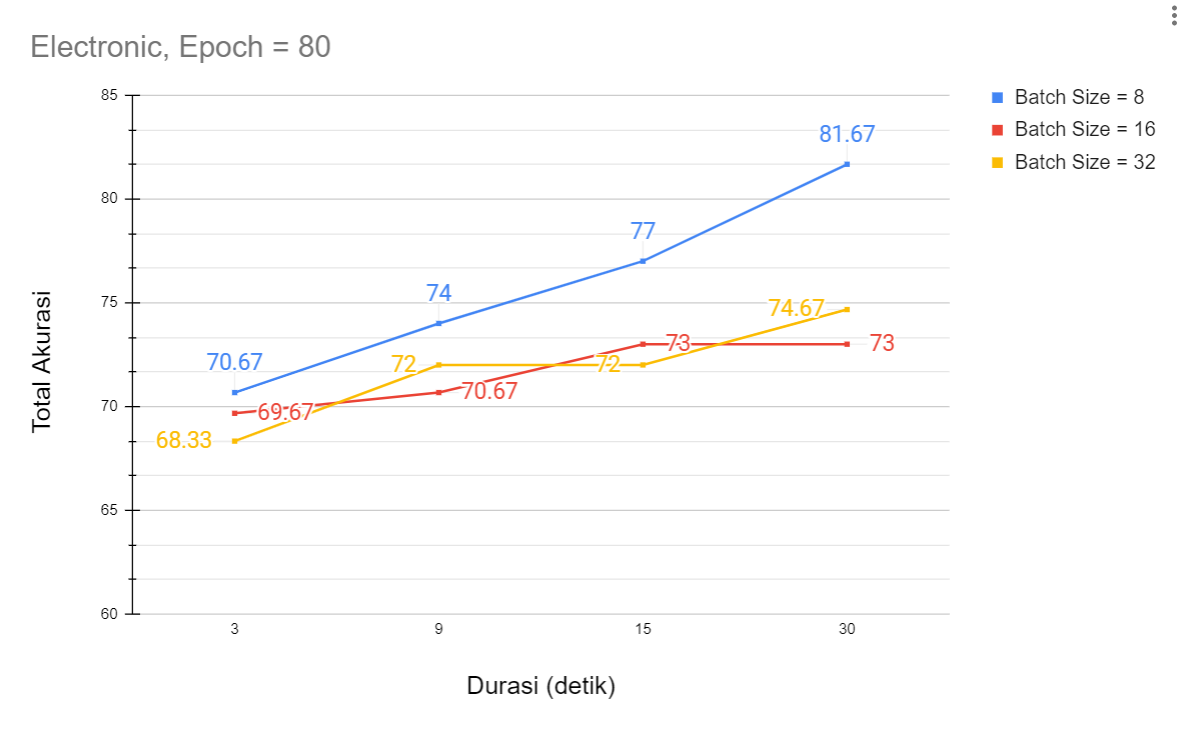
\includegraphics[width=0.9\textwidth]{gambar/e80_chart_sum accuracy_electronic}
			
			% Ubah dengan keterangan gambar yang diinginkan
			\caption{Grafik Garis Akurasi Simulasi Genre Elektronik Dengan Epoch = 80}
			\label{fig:elecsumcharte80}
		\end{figure}
		
		Pada Gambar 4.22 dapat terlihat bahwa akurasi simulasi genre Elektronik dengan \emph{epoch} = 80 pada masing-masing durasi (3 detik, 9 detik, 15 detik, dan 30 detik) tidak pernah mengalami penurunan. Sempat terjadi stagnasi pada \emph{batch size} = 32 dan durasi 9 ke 15 detik, serta pada \emph{batch size} = 16 dan durasi 15 ke 30 detik. Selain itu, terjadi kenaikan pada sisanya. Pada Tabel 4.26 dapat diketahui bahwa rata-rata tertinggi didapat pada \emph{batch size} = 8 dan rata-rata terendah didapat \emph{batch size} = 16.
		
		\begin{longtable}[c]{|c|c|c|c|}
			\caption{Tabel Hasil Simulasi Genre Elektronik Dengan Epoch = 100}
			\label{tab:my-table}\\
			\hline
			\textbf{Batch Size} & \textbf{Durasi (detik)} & \textbf{Total Akurasi} & \textbf{Rata-rata (\%)}       \\ \hline
			\endfirsthead
			%
			\endhead
			%
			\multirow{4}{*}{8}  & 3                       & 69.67                  & \multirow{4}{*}{74.6675} \\ \cline{2-3}
			& 9                       & 74.67                  &                          \\ \cline{2-3}
			& 15                      & 76.33                  &                          \\ \cline{2-3}
			& 30                      & 78                     &                          \\ \hline
			\multirow{4}{*}{16} & 3                       & 69.33                  & \multirow{4}{*}{74.5825} \\ \cline{2-3}
			& 9                       & 76.33                  &                          \\ \cline{2-3}
			& 15                      & 76                     &                          \\ \cline{2-3}
			& 30                      & 76.67                  &                          \\ \hline
			\multirow{4}{*}{32} & 3                       & 75.33                  & \multirow{4}{*}{76.5}    \\ \cline{2-3}
			& 9                       & 75.67                  &                          \\ \cline{2-3}
			& 15                      & 75.67                  &                          \\ \cline{2-3}
			& 30                      & 79.33                  &                          \\ \hline
		\end{longtable}
		
		\begin{figure}[H]
			\centering
			
			% Ubah dengan nama file gambar dan ukuran yang akan digunakan
			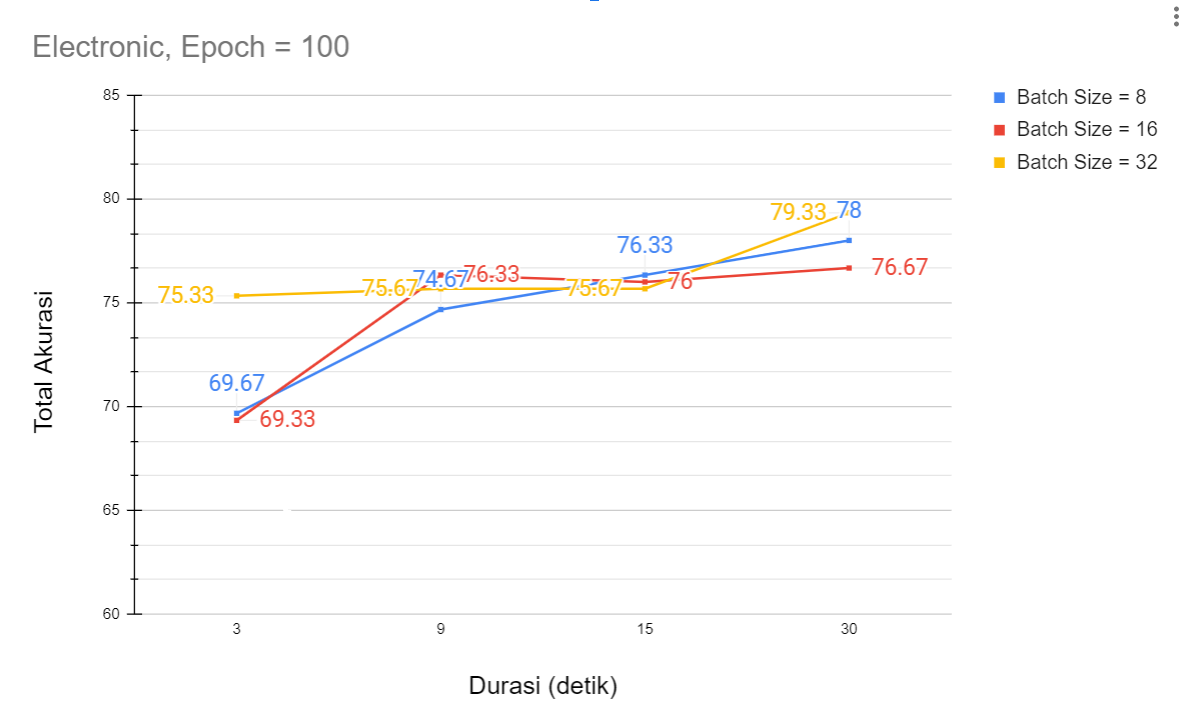
\includegraphics[width=\textwidth]{gambar/e100_chart_sum accuracy_electronic}
			
			% Ubah dengan keterangan gambar yang diinginkan
			\caption{Grafik Garis Akurasi Simulasi Genre Elektronik Dengan Epoch = 100}
			\label{fig:elecsumcharte100}
		\end{figure}
		
		Pada Gambar 4.23 dapat terlihat bahwa akurasi simulasi genre Elektronik dengan \emph{epoch} = 80 pada masing-masing durasi (3 detik, 9 detik, 15 detik, dan 30 detik) terjadi kenaikan, stagnasi, dan penurunan. Sempat terjadi stagnasi pada \emph{batch size} = 32 dan durasi 9 ke 15 detik. Sempat juga terjadi penurunan pada \emph{batch size} = 16 dan durasi 9 ke 15 detik. Selain itu, terjadi kenaikan pada sisanya. Pada Tabel 4.27 dapat diketahui bahwa rata-rata tertinggi didapat pada \emph{batch size} = 32 dan rata-rata terendah didapat \emph{batch size} = 16.
		
		Pada genre Elektronik didapat rata-rata tertinggi pada \emph{epoch} = 100 dan \emph{batch size} = 32 dengan hasil total akurasi 76,5\%. Rata-rata terendah didapat pada \emph{epoch} = 80 dan \emph{batch size} = 16 dengan hasil total akurasi 71,585\%. Selain itu, juga didapat grafik paling stabil yaitu pada \emph{epoch} = 100 dan \emph{batch size} = 32 dikarenakan tidak terjadi penurunan dan memiliki selisih total akurasi antara durasi 30 dengan 3 detik yang paling sedikit yaitu sebanyak 4\%. Didapat pula grafik yang memiliki kenaikan paling drastis antara masing-masing, yaitu pada \emph{epoch} = 80 dan \emph{batch size} = 8. Terakhir, didapat grafik yang memiliki perkembangan terburuk, yaitu pada \emph{epoch} = 100 dan \emph{batch size} = 16 dikarenakan sempat terjadi penurunan pada durasi 9 ke 15 detik.
		
	\item Rock
		\begin{longtable}[c]{|c|c|c|c|}
			\caption{Tabel Hasil Simulasi Genre Rock Dengan Epoch = 80}
			\label{tab:my-table}\\
			\hline
			\textbf{Batch Size} & \textbf{Durasi (detik)} & \textbf{Total Akurasi} & \textbf{Rata-rata (\%)}       \\ \hline
			\endfirsthead
			%
			\endhead
			%
			\multirow{4}{*}{8}  & 3                       & 62                     & \multirow{4}{*}{63.5825} \\ \cline{2-3}
			& 9                       & 62.67                  &                          \\ \cline{2-3}
			& 15                      & 63.33                  &                          \\ \cline{2-3}
			& 30                      & 66.33                  &                          \\ \hline
			\multirow{4}{*}{16} & 3                       & 65.33                  & \multirow{4}{*}{67.8325} \\ \cline{2-3}
			& 9                       & 67                     &                          \\ \cline{2-3}
			& 15                      & 68                     &                          \\ \cline{2-3}
			& 30                      & 71                     &                          \\ \hline
			\multirow{4}{*}{32} & 3                       & 63                     & \multirow{4}{*}{64.585}  \\ \cline{2-3}
			& 9                       & 63.67                  &                          \\ \cline{2-3}
			& 15                      & 64                     &                          \\ \cline{2-3}
			& 30                      & 67.67                  &                          \\ \hline
		\end{longtable}
		
		\begin{figure}[H]
			\centering
			
			% Ubah dengan nama file gambar dan ukuran yang akan digunakan
			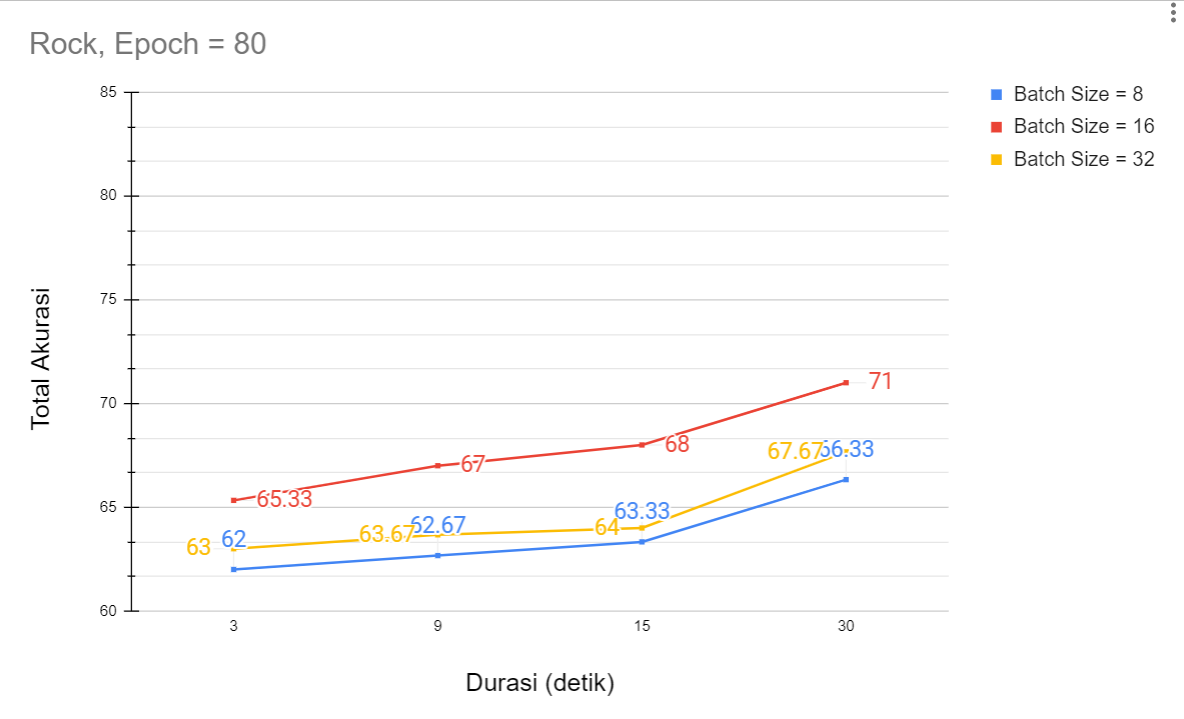
\includegraphics[width=\textwidth]{gambar/e80_chart_sum accuracy_rock}
			
			% Ubah dengan keterangan gambar yang diinginkan
			\caption{Grafik Garis Akurasi Simulasi Genre Rock Dengan Epoch = 80}
			\label{fig:rocksumcharte80}
		\end{figure}
		
		Pada Gambar 4.24 dapat terlihat bahwa akurasi simulasi genre Rock dengan \emph{epoch} = 80 pada masing-masing durasi (3 detik, 9 detik, 15 detik, dan 30 detik) tidak pernah mengalami penurunan dan stagnasi, hanya kenaikan. Pada Tabel 4.28 dapat diketahui bahwa rata-rata tertinggi didapat pada \emph{batch size} = 16 dan rata-rata terendah didapat \emph{batch size} = 8.
		
		\begin{longtable}[c]{|c|c|c|c|}
			\caption{Tabel Hasil Simulasi Genre Rock Dengan Epoch = 100}
			\label{tab:my-table}\\
			\hline
			\textbf{Batch Size} & \textbf{Durasi (detik)} & \textbf{Total Akurasi} & \textbf{Rata-rata (\%)}       \\ \hline
			\endfirsthead
			%
			\endhead
			%
			\multirow{4}{*}{8}  & 3                       & 63                     & \multirow{4}{*}{68.3325} \\ \cline{2-3}
			& 9                       & 66.33                  &                          \\ \cline{2-3}
			& 15                      & 69                     &                          \\ \cline{2-3}
			& 30                      & 75                     &                          \\ \hline
			\multirow{4}{*}{16} & 3                       & 68.67                  & \multirow{4}{*}{69}      \\ \cline{2-3}
			& 9                       & 68                     &                          \\ \cline{2-3}
			& 15                      & 68                     &                          \\ \cline{2-3}
			& 30                      & 71.33                  &                          \\ \hline
			\multirow{4}{*}{32} & 3                       & 61.33                  & \multirow{4}{*}{62.665}  \\ \cline{2-3}
			& 9                       & 61.33                  &                          \\ \cline{2-3}
			& 15                      & 62.33                  &                          \\ \cline{2-3}
			& 30                      & 65.67                  &                          \\ \hline
		\end{longtable}
		
		\begin{figure}[H]
			\centering
			
			% Ubah dengan nama file gambar dan ukuran yang akan digunakan
			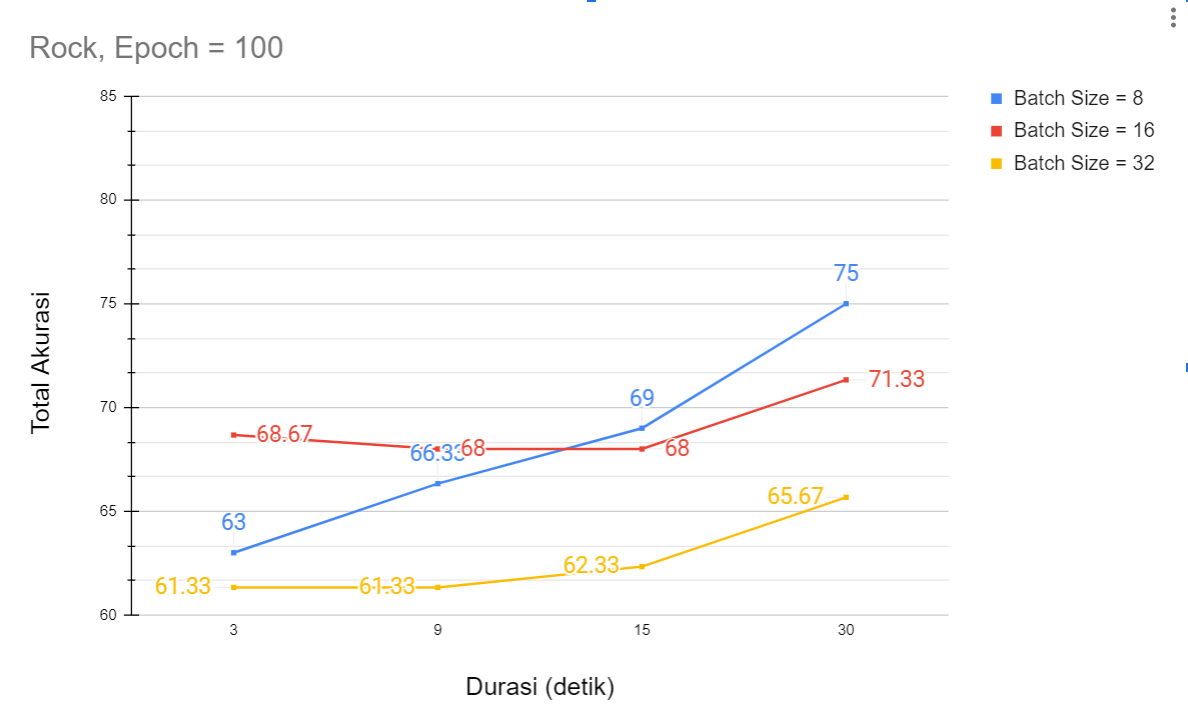
\includegraphics[width=\textwidth]{gambar/e100_chart_sum accuracy_rock}
			
			% Ubah dengan keterangan gambar yang diinginkan
			\caption{Grafik Garis Akurasi Simulasi Genre Rock Dengan Epoch = 100}
			\label{fig:rocksumcharte100}
		\end{figure}
		
		Pada Gambar 4.25 dapat terlihat bahwa akurasi simulasi genre Rock dengan \emph{epoch} = 100 pada masing-masing durasi (3 detik, 9 detik, 15 detik, dan 30 detik) pernah mengalami penurunan dan stagnasi. Sempat terjadi stagnasi pada \emph{batch size} = 16 dan durasi 9 ke 15 detik, serta pada \emph{batch size} = 32 dan durasi 3 ke 9 detik. Penurunan juga terjadi pada \emph{batch size} = 16 dan durasi 3 ke 9 detik.  Selain itu, terjadi kenaikan pada sisanya. Pada Tabel 4.29 dapat diketahui bahwa rata-rata tertinggi didapat pada \emph{batch size} = 16 dan rata-rata terendah didapat \emph{batch size} = 32.
		
		Pada genre Rock didapat rata-rata tertinggi pada \emph{epoch} = 100 dan \emph{batch size} = 16 dengan hasil total akurasi 69\%. Rata-rata terendah didapat pada \emph{epoch} = 100 dan \emph{batch size} = 32 dengan hasil total akurasi 62,665\%. Selain itu, juga didapat grafik paling stabil yaitu pada \emph{epoch} = 80 dan \emph{batch size} = 8 dikarenakan tidak terjadi penurunan dan memiliki selisih total akurasi antara durasi 30 dengan 3 detik yang paling sedikit yaitu sebanyak 4,33\%. Didapat pula grafik yang memiliki kenaikan paling drastis antara masing-masing, yaitu pada \emph{epoch} = 100 dan \emph{batch size} = 8. Terakhir, didapat grafik yang memiliki perkembangan terburuk, yaitu pada \emph{epoch} = 100 dan \emph{batch size} = 16 dikarenakan sempat terjadi penurunan pada durasi 9 ke 15 detik, meskipun memiliki rata-rata akurasi tertinggi, yaitu 69\%.
		
	\item Folk
		\begin{longtable}[c]{|c|c|c|c|}
			\caption{Tabel Hasil Simulasi Genre Folk Dengan Epoch = 80}
			\label{tab:my-table}\\
			\hline
			\textbf{Batch Size} & \textbf{Durasi (detik)} & \textbf{Total Akurasi} & \textbf{Rata-rata (\%)}       \\ \hline
			\endfirsthead
			%
			\endhead
			%
			\multirow{4}{*}{8}  & 3                       & 63.67                  & \multirow{4}{*}{68.0025} \\ \cline{2-3}
			& 9                       & 67.67                  &                          \\ \cline{2-3}
			& 15                      & 70                     &                          \\ \cline{2-3}
			& 30                      & 70.67                  &                          \\ \hline
			\multirow{4}{*}{16} & 3                       & 70                     & \multirow{4}{*}{70.335}  \\ \cline{2-3}
			& 9                       & 70.67                  &                          \\ \cline{2-3}
			& 15                      & 69.67                  &                          \\ \cline{2-3}
			& 30                      & 71                     &                          \\ \hline
			\multirow{4}{*}{32} & 3                       & 66.67                  & \multirow{4}{*}{68.0025} \\ \cline{2-3}
			& 9                       & 67                     &                          \\ \cline{2-3}
			& 15                      & 69.67                  &                          \\ \cline{2-3}
			& 30                      & 68.67                  &                          \\ \hline
		\end{longtable}
		
		\begin{figure}[H]
			\centering
			
			% Ubah dengan nama file gambar dan ukuran yang akan digunakan
			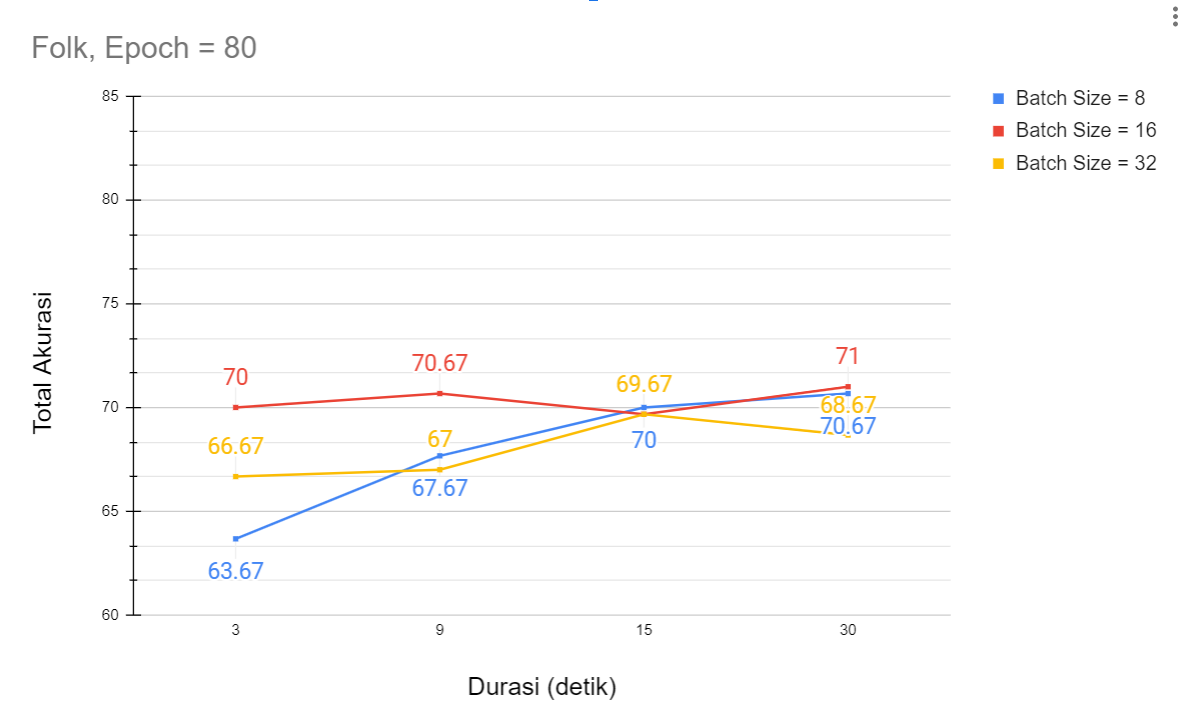
\includegraphics[width=\textwidth]{gambar/e80_chart_sum accuracy_folk}
			
			% Ubah dengan keterangan gambar yang diinginkan
			\caption{Grafik Garis Akurasi Simulasi Genre Folk Dengan Epoch = 80}
			\label{fig:folksumcharte80}
		\end{figure}
		
		Pada Gambar 4.26 dapat terlihat bahwa akurasi simulasi genre Folk dengan \emph{epoch} = 80 pada masing-masing durasi (3 detik, 9 detik, 15 detik, dan 30 detik) pernah mengalami penurunan, namun tidak pernah terjadi stagnasi. Sempat terjadi penurunan pada \emph{batch size} = 32 dan durasi 15 ke 30 detik, serta pada \emph{batch size} = 16 dan durasi 9 ke 15 detik. Selain itu, terjadi kenaikan pada sisanya. Pada Tabel 4.30 dapat diketahui bahwa rata-rata tertinggi didapat pada \emph{batch size} = 16 dan rata-rata terendah didapat kedua \emph{batch size} = 8 dan 32.
		
		\begin{longtable}[c]{|c|c|c|c|}
			\caption{Tabel Hasil Simulasi Genre Folk Dengan Epoch = 100}
			\label{tab:my-table}\\
			\hline
			\textbf{Batch Size} & \textbf{Durasi (detik)} & \textbf{Total Akurasi} & \textbf{Rata-rata (\%)}       \\ \hline
			\endfirsthead
			%
			\endhead
			%
			\multirow{4}{*}{8}  & 3                       & 68                     & \multirow{4}{*}{68.25}   \\ \cline{2-3}
			& 9                       & 70.67                  &                          \\ \cline{2-3}
			& 15                      & 67.66                  &                          \\ \cline{2-3}
			& 30                      & 66.67                  &                          \\ \hline
			\multirow{4}{*}{16} & 3                       & 60                     & \multirow{4}{*}{64.8325} \\ \cline{2-3}
			& 9                       & 66.33                  &                          \\ \cline{2-3}
			& 15                      & 68.67                  &                          \\ \cline{2-3}
			& 30                      & 64.33                  &                          \\ \hline
			\multirow{4}{*}{32} & 3                       & 68.67                  & \multirow{4}{*}{69.8325} \\ \cline{2-3}
			& 9                       & 71.33                  &                          \\ \cline{2-3}
			& 15                      & 70.33                  &                          \\ \cline{2-3}
			& 30                      & 69                     &                          \\ \hline
		\end{longtable}
		
		\begin{figure}[H]
			\centering
			
			% Ubah dengan nama file gambar dan ukuran yang akan digunakan
			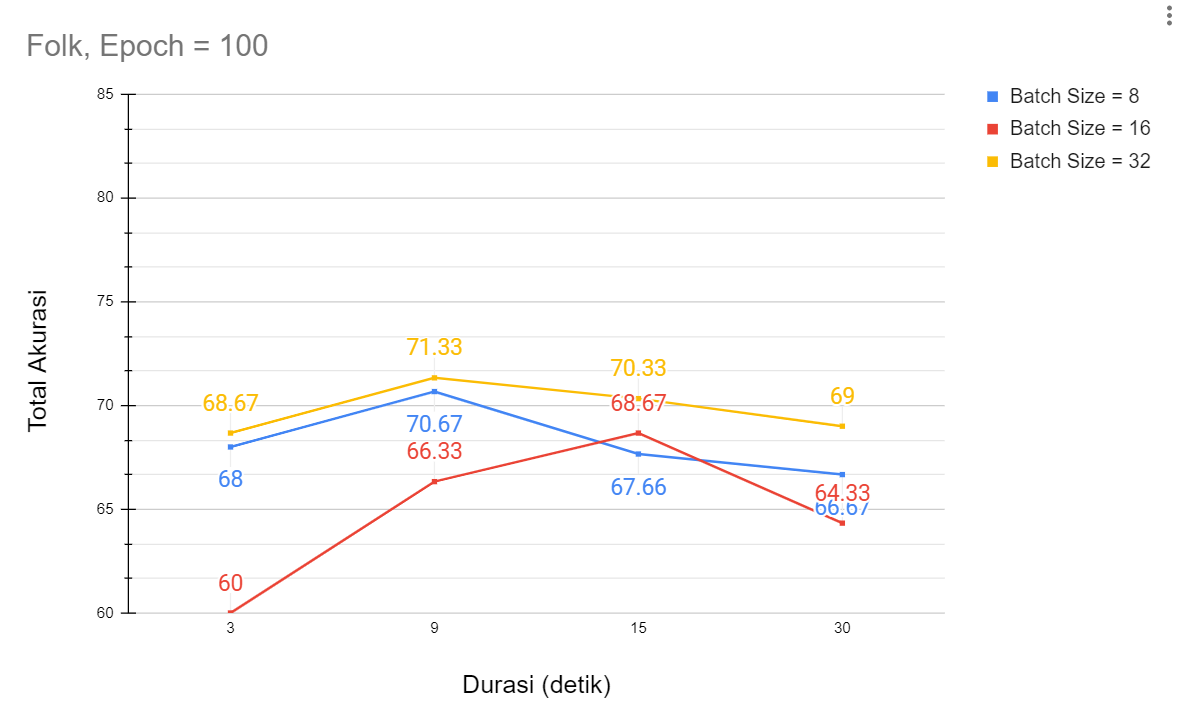
\includegraphics[width=\textwidth]{gambar/e100_chart_sum accuracy_folk}
			
			% Ubah dengan keterangan gambar yang diinginkan
			\caption{Grafik Garis Akurasi Simulasi Genre Folk Dengan Epoch = 100}
			\label{fig:folksumcharte100}
		\end{figure}
		
		Pada Gambar 4.27 dapat terlihat bahwa akurasi simulasi genre Folk dengan \emph{epoch} = 100 pada masing-masing durasi (3 detik, 9 detik, 15 detik, dan 30 detik) pernah mengalami penurunan, namun tidak terjadi stagnasi. Banyak terjadi penurunan, contohnya pada \emph{batch size} = 8 dari durasi 9 ke 30 detik selalu mengalami penurunan, pada \emph{batch size} = 16 dan durasi 15 ke 30 detik, serta pada \emph{batch size} = 32 dari durasi 9 ke 30 detik selalu mengalami penurunan.  Selain itu, terjadi kenaikan pada sisanya. Pada Tabel 4.31 dapat diketahui bahwa rata-rata tertinggi didapat pada \emph{batch size} = 32 dan rata-rata terendah didapat \emph{batch size} = 16.
		
		Pada genre Folk Didapat rata-rata tertinggi pada \emph{epoch} = 80 dan \emph{batch size} = 16 dengan hasil total akurasi 70,335\%. Rata-rata terendah didapat pada \emph{epoch} = 100 dan \emph{batch size} = 16 dengan hasil total akurasi 64,8325\%. Selain itu, juga didapat grafik paling stabil yaitu pada \emph{epoch} = 80 dan \emph{batch size} = 8 dikarenakan tidak terjadi penurunan dan memiliki selisih total akurasi antara durasi 30 dengan 3 detik yang paling sedikit yaitu sebanyak 7\%. Grafik ini juga merupakan yang memiliki kenaikan paling drastis seiring bertambahnya durasi. Terakhir, pada \emph{epoch} = 100 semua kasus \emph{batch size} mengalami penurunan yang lebih banyak dibandingkan dengan \emph{epoch} = 80 serta pada genre lainnya. 
		
\end{enumerate}

Setelah dilihat analisis pada masing-masing genre diatas maka dapat ditarik beberapa poin. Pertama, genre Elektronik memiliki hasil simulasi yang terbaik dikarenakan memiliki rata-rata yang paling tinggi serta grafik yang stabil. Kedua, genre Folk memiliki hasil simulasi yang paling tidak stabil dibandingkan dengan Rock dan Elektronik dikarenakan banyaknya terjadi penurunan seiring pertambahan durasi pada input data. Ketiga, tidak ada kaitannya antara tingginya rata-rata akurasi dengan kestabilan grafik.

\section{Total Akurasi Simulasi}
\label{sec:totalakurasi}

Pada subbab sebelumnya telah ditunjukkan mengenai hasil klasifikasinya yang berupa daftar 3 subgenre tertinggi dengan masing-masing presentasenya. Pada tahap ini dilakukan perhitungan akurasi berdasarkan pada seberapa akurat sistem dalam mengklasifikasikan suatu trek musik dengan true label subgenre tertentu dengan cara menjumlahkan akurasi semua kasus saat true label mendapatkan urutan klasifikasi ke 1 sampai 3. Untuk melakukan pengujian ini juga menggunakan dataset dari Free Music Archive (FMA) dengan jumlah 100 trek tiap subgenrenya, yaitu total 900 trek. Dataset untuk simulasi ini berbeda dengan dataset yang digunakan saat melakukan training. Berikut untuk tabel total akurasinya dapat dilihat melalui Tabel 4.1.

\begin{longtable}[Hc]{|c|c|c|c|}
	\hline
	\multicolumn{1}{|l|}{\textbf{Epoch}} & \multicolumn{1}{l|}{\textbf{Batch Size}} & \multicolumn{1}{l|}{\textbf{Durasi (detik)}} & \multicolumn{1}{l|}{\textbf{Total Akurasi}} \\ \hline
	\endfirsthead
	%
	\endhead
	%
	\multirow{12}{*}{80}                 & \multirow{4}{*}{8}                       & 3                                            & 65,44\%                                     \\ \cline{3-4} 
	&                                          & 9                                            & 68,11\%                                     \\ \cline{3-4} 
	&                                          & 15                                           & 70,11\%                                     \\ \cline{3-4} 
	&                                          & 30                                           & 72,89\%                                     \\ \cline{2-4} 
	& \multirow{4}{*}{16}                      & 3                                            & 68,33\%                                     \\ \cline{3-4} 
	&                                          & 9                                            & 69,44\%                                     \\ \cline{3-4} 
	&                                          & 15                                           & 70,22\%                                     \\ \cline{3-4} 
	&                                          & 30                                           & 71,67\%                                     \\ \cline{2-4} 
	& \multirow{4}{*}{32}                      & 3                                            & 66\%                                     \\ \cline{3-4} 
	&                                          & 9                                            & 67,56\%                                     \\ \cline{3-4} 
	&                                          & 15                                           & 68,56\%                                     \\ \cline{3-4} 
	&                                          & 30                                           & 70,33\%                                     \\ \hline
	\multirow{12}{*}{100}                & \multirow{4}{*}{8}                       & 3                                            & 66,22\%                                     \\ \cline{3-4} 
	&                                          & 9                                            & 70,56\%                                     \\ \cline{3-4} 
	&                                          & 15                                           & 71\%                                        \\ \cline{3-4} 
	&                                          & 30                                           & 73,22\%                                     \\ \cline{2-4} 
	& \multirow{4}{*}{16}                      & 3                                            & 66\%                                     \\ \cline{3-4} 
	&                                          & 9                                            & 68,78\%                                     \\ \cline{3-4} 
	&                                          & 15                                           & 69\%                                        \\ \cline{3-4} 
	&                                          & 30                                           & 71,44\%                                     \\ \cline{2-4} 
	& \multirow{4}{*}{32}                      & 3                                            & 68,44\%                                     \\ \cline{3-4} 
	&                                          & 9                                            & 69,44\%                                     \\ \cline{3-4} 
	&                                          & 15                                           & 69,44\%                                     \\ \cline{3-4} 
	&                                          & 30                                           & 71,33\%                                     \\ \hline
	\caption{Tabel Total Akurasi Simulasi}
	\label{tab:my-table}\\
\end{longtable}

Untuk melihat perbandingan total akurasi secara lebih jelas, telah dibuat grafik garis seperti yang tertera pada Gambar 4.22 untuk Epoch = 80 dan Gambar 4.23 untuk Epoch = 100. Garis warna biru untuk menunjukkan perkembangan akurasi seiring bertambahnya durasi dari \emph{batch size} = 8, garis merah untuk \emph{batch size} = 16, dan garis kuning untuk \emph{batch size} = 32.

\begin{figure}[H]
	\centering
	
	% Ubah dengan nama file gambar dan ukuran yang akan digunakan
	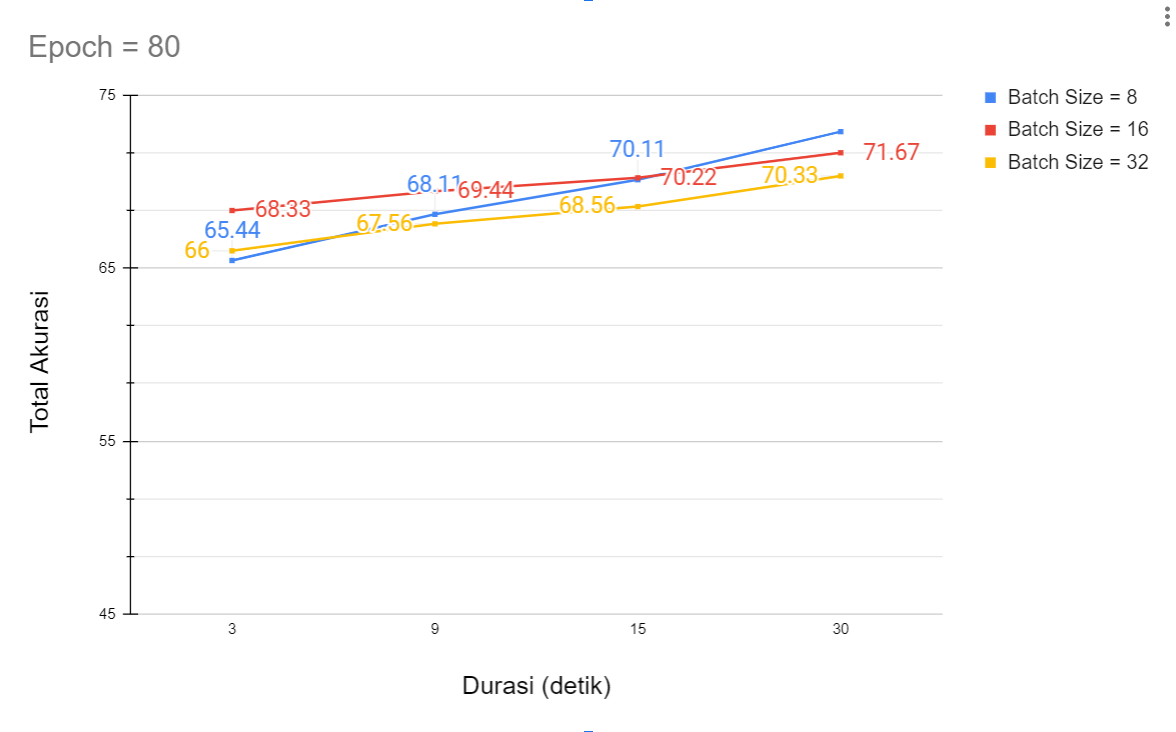
\includegraphics[width=0.95\textwidth]{gambar/e80_chart_sum accuracy}
	
	% Ubah dengan keterangan gambar yang diinginkan
	\caption{Grafik Garis Total Akurasi Simulasi Dengan Epoch = 80}
	\label{fig:sumcharte80}
\end{figure}

Pada Gambar 4.28 dapat terlihat bahwa total akurasi simulasi dengan \emph{epoch} = 80 pada masing-masing durasi (3 detik, 9 detik, 15 detik, dan 30 detik) tidak pernah mengalami penurunan. Pada semua \emph{batch size} hanya ada kenaikan seiring bertambahnya durasi input trek.

\begin{figure}[H]
	\centering
	
	% Ubah dengan nama file gambar dan ukuran yang akan digunakan
	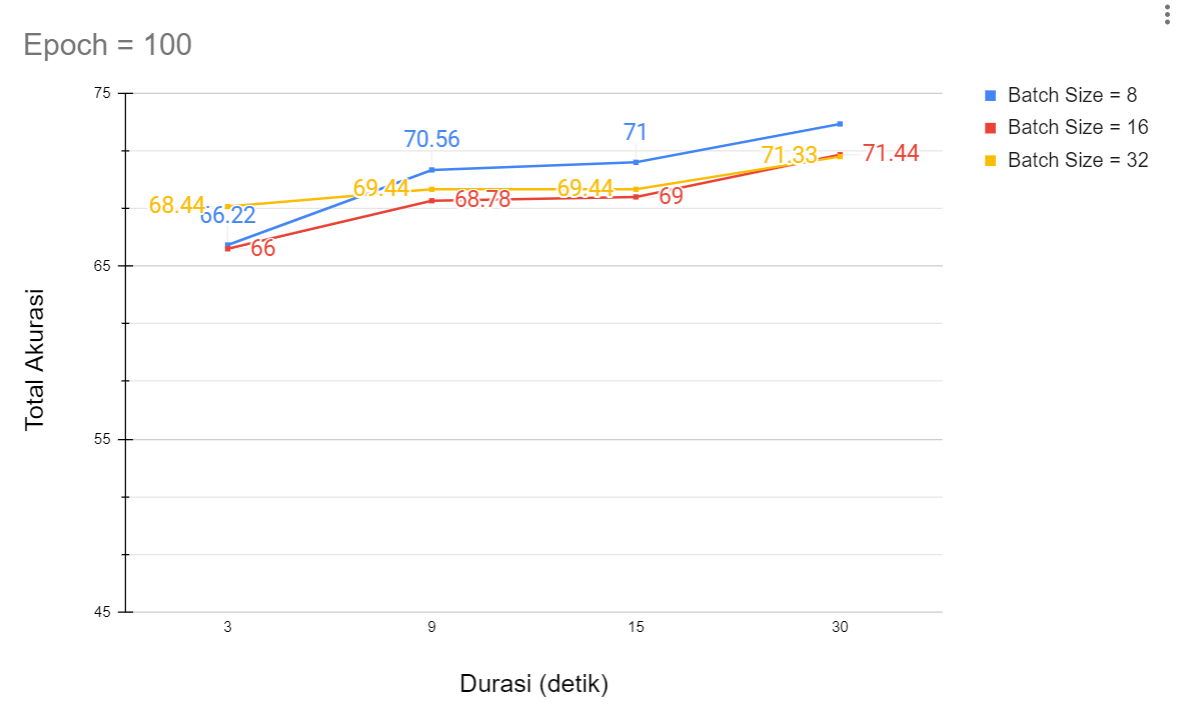
\includegraphics[width=0.95\textwidth]{gambar/e100_chart_sum accuracy}
	
	% Ubah dengan keterangan gambar yang diinginkan
	\caption{Grafik Garis Total Akurasi Simulasi Dengan Epoch = 100}
	\label{fig:sumcharte100}
\end{figure}

Pada Gambar 4.29 dapat terlihat bahwa total akurasi simulasi dengan \emph{epoch} = 100 pada masing-masing durasi (3 detik, 9 detik, 15 detik, dan 30 detik) tidak pernah mengalami penurunan, namun sempat terjadi stagnasi. Stagnasi terjadi pada \emph{batch size} = 32 dan durasi 9 ke 15 detik, yaitu dengan akurasi sebesar 69,44\%. Selain itu, pada semua \emph{batch size} dan durasi hanya terjadi kenaikan.

Dilihat dari grafik garis pada Gambar 4.28 dan Gambar 4.29 dapat dilihat pada masing-masing parameter \emph{Epoch} dan \emph{Batch Size} selalu mengalami peningkatan seiring menambahnya durasi trek input. Dari sini dapat dikatakan bahwa semakin panjangnya durasi trek maka semakin akurat pula sistem dalam mengklasifikasikan trek tersebut sesuai dengan true labelnya.

\section{Komparasi Penelitian Terkait}
\label{sec:komparasipenelitian}

Langkah terakhir untuk menilai performa sistem yang telah dibuat pada penelitian ini secara objektif adalah untuk membandingkannya dengan penelitian-penelitian terdahulu. Penelitian ini menggunakan total 9 subgenre yang berisi 3 subgenre tiap masing-masing genre. Penelitian oleh Quinto dkk. \citep{quinto} menggunakan 3 subgenre dari genre musik jazz, Tsatsishvili \cite{tsatsishvili} menggunakan 7 subgenre dari genre musik heavy metal, dan Mulder \citep{Mulder2014AutomaticCO} menggunakan 17 subgenre dari genre musik heavy metal. Ketiga contoh ini menggunakan subgenre dari kategori genre yang sama, sedangkan pada penelitian ini mencoba menggunakan genre yang berbeda-beda. Akurasi training model tertinggi yang didapat pada penelitian ini adalah sebesar 47,69\% pada \emph{epoch} = 100 dan \emph{batch size} = 8. Dari nilai akurasi masih lebih rendah dari penelitian oleh Quinto dkk. yang dimana akurasi tertingginya didapat dari metode LSTM, yaitu dengan nilai 89,824\% meskipun jumlah class yang digunakan hanya 3 (bergantung pada jumlah subgenrenya). Namun, penelitian ini mendapatkan akurasi yang lebih tinggi dibandingkan dengan penelitian oleh Tsatsishvili dan Mulder yang dimana masing-masing mendapatkan akurasi tertingginya 45,7\% dan 28\% yang dimana Tsatsishvili menggunakan 7 class dan Mulder menggunakan 17 class.

Selain itu, penelitian ini bertujuan untuk membuat sistem yang dapat merekomendasikan 3 subgenre tertinggi yang paling masuk akal berdasarkan input musiknya yang dimana pada ketiga penelitian terdahulu tersebut hanya berfokus pada klasifikasi spesifik 1 subgenre. Kemudian, perbedaan yang paling akhir adalah penelitian ini membuat sistem yang dapat mengklasifikasikan musik dengan durasi yang lebih fleksibel, yaitu dengan durasi kelipatan dari 3 detik (contoh: 3, 6, 9, 12, 15, dan seterusnya). Apabila durasi lebih dari 3 detik namun bukan kelipatan dari 3 maka akan input trek akan dianggap memiliki durasi kelipatan 3 sebelumnya (contoh: input trek dengan durasi 10 detik maka akan dianggap sebagai 9 detik). Sedangkan, ketiga penelitian terdahulu tidak mengimplementasikan sistem yang dapat mengklasifikasikan input trek dengan durasi yang fleksibel.
  \cleardoublepage

  % Bab 5 penutup
  \chapter{PENUTUP}
\label{chap:penutup}

% Ubah bagian-bagian berikut dengan isi dari penutup

\section{Kesimpulan}
\label{sec:kesimpulan}

Berdasarkan hasil pengujian yang dilakukan penulis berhasil menerapkan sebuah sistem untuk mengklasifikasikan genre dan subgenre musik dengan MFCC sebagai fiturnya serta menggunakan CNN sebagai algoritmanya. Untuk lebih dalamnya dapat dilihat sebagai berikut:

\begin{enumerate}[nolistsep]

  \item Sistem membuktikan bahwa algoritma CNN dapat digunakan untuk mengklasifikasikan subgenre dari suatu input data musik.

  \item Akurasi training tertinggi didapat pada Batch Size = 32, dan Epoch = 100 dengan hasil 46,39\%.

  \item Berdasarkan hasil dari Confusion Matrix, didapatkan bahwa sistem dapat mengklasifikasikan subgenre Chiptune dengan baik, namun sebaliknya pengklasifikasian subgenre Psych Folk masih sering disalah artikan sebagai subgenre lainnya, seperti Post Rock, Loud Rock, Noise Rock, dan Freak Folk.
  
  \item Terbukti output dari sistem dapat mengklasifikasikan suatu input data musik ke tiga terbesar subgenrenya yang paling masuk akal.
  
  \item Durasi input musik memiliki peran besar dalam meningkatkan akurasi dari klasifikasi. Berdasarkan Gambar 4.22 dan Gambar 4.23, didapatkan akurasi tertinggi pada input musik dengan durasi 30 detik.

\end{enumerate}

\section{Saran}
\label{chap:saran}

Untuk pengembangan lebih lanjut pada penelitian ini terdapat beberapa saran yang mungkin bisa dilakukan pada penelitian selanjutnya, yaitu antara lain:

\begin{enumerate}[nolistsep]

  \item Menggunakan dataset yang memiliki lebih banyak serta lebih dapat diandalkan agar dapat menguji coba sistem dengan lebih banyak subgenre, jumlah trek, serta durasi yang lebih panjang pula.

  \item Menggunakan fitur-fitur audio lain selain MFCC agar dapat menguji coba efektifitas masing-masing fitur audio dalam pengklasifikasian subgenre musik.

  \item Menggunakan algoritma machine learning maupun deep learning yang lain untuk menguji efisiensi dari masing-masing algoritma dalam pengklasifikasian subgenre musik.

\end{enumerate}

  \cleardoublepage

  % Daftar pustaka
  \renewcommand\bibname{DAFTAR PUSTAKA}
  \addcontentsline{toc}{chapter}{\bibname}
  \bibliographystyle{apa}
  \bibliography{pustaka/pustaka.bib}
  \cleardoublepage

  % Biografi penulis
  \begin{center}
  \Large
  \textbf{BIOGRAFI PENULIS}
\end{center}

\addcontentsline{toc}{chapter}{BIOGRAFI PENULIS}

\vspace{2ex}

\begin{wrapfigure}{L}{0.3\textwidth}
  \centering
  \vspace{-3ex}
  % Ubah file gambar berikut dengan file foto dari mahasiswa
  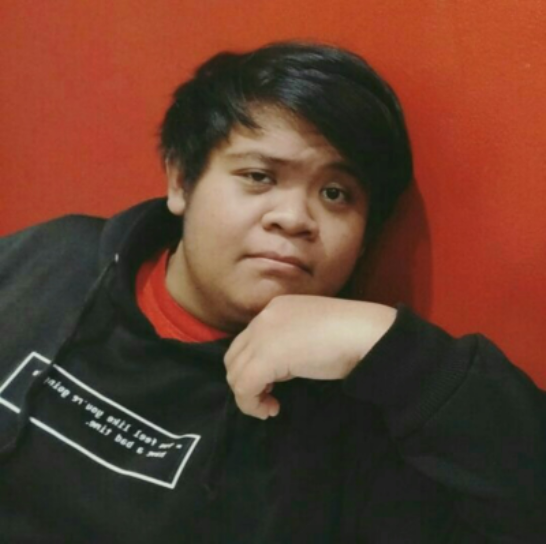
\includegraphics[width=0.3\textwidth]{gambar/profil.png}
  \vspace{-4ex}
\end{wrapfigure}

% Ubah kalimat berikut dengan biografi dari mahasiswa
Dimas Iqbal Fahreza atau yang lebih akrab disapa Dif, lahir di Bandar Lampung pada tanggal 6 Oktober 2000. Merupakan anak kedua dari dua bersaudara. Penulis lulus dari SMP Negeri 5 Yogyakarta dan kemudian melanjutkan ke SMA Negeri 2 Yogyakarta. Penulis merupakan salah satu mahasiswa dari Departemen Teknik Komputer Surabaya, Fakultas Teknologi Elektro dan Informatika Cerdas, Institut Teknologi Sepuluh Nopember. Dalam masa kuliah, penulis memiliki \emph{passion} terhadap bidang \emph{Game Development}. Selain itu, penulis juga memiliki hobi bermusik, baik dari memainkan alat musik piano, maupun membuat musik atau \emph{sound effects} untuk segala keperluan pengembangan gim. Penulis juga aktif ikut serta dalam kompetisi \emph{Game Development}. Kompetisi yang pernah dimenangkan adalah juara 3 GameDev HOLOGY 3.0. UB, dan menjadi finalis di MAGE ITS. Hingga sampai detik buku ini disusun, penulis masih memperjuangkan \emph{passion}-nya di bidang \emph{Game Development} dengan mengembangkan sebuah gim \emph{indie} pada tim yang telah didirikan sejak tahun 2021.

  \cleardoublepage

\end{document}
